\documentclass[pldi,preprint]{sigplanconf-pldi16}

\usepackage{amsmath,amssymb,amsopn,amsthm}
\usepackage[T1]{fontenc}
\usepackage{algorithmicx,algorithm}
\usepackage[noend]{algpseudocode}
\usepackage{multirow}
\usepackage{cleveref}
\usepackage{graphicx}
\usepackage[usenames,dvipsnames]{xcolor}
\usepackage{verbatim}
\usepackage{relsize}
\usepackage{ifluatex}
%\usepackage{stfloats}

\usepackage{tikz}
\usetikzlibrary{fit,positioning,patterns,shapes,shapes.multipart}
\usepackage{pgfplots}
\usepackage{pgfplotstable}
\pgfplotsset{compat=1.12} 

\newcommand\newterm[1]{{\it #1}}
\newcommand\R{\mathbb{R}}
\newcommand\N{\mathbb{N}}
\newcommand\B{\mathbb{B}}
\newcommand\T{\mathcal{T}}
\renewcommand\S{\mathcal{S}}

\newcommand\lspan[2]{\multicolumn{#1}{@{}l}{#2}}
\newcommand\cspan[2]{\multicolumn{#1}{@{}c}{#2}}

\makeatletter
\newcommand{\LeftEqNo}{\let\veqno\@@leqno}
\makeatother

\newcommand\limplies{\rightarrow}
\newcommand\liff{\leftrightarrow}

\newcommand\exampleTitle{
\bigskip\noindent
\begin{tikzpicture}
  \draw (0,0) -- (5mm,0)
    node(e)[draw,rectangle,rounded corners=.7em,right] {\bf Example};
  \draw (e) -- (\columnwidth,0);
\end{tikzpicture}%
\medskip%
}

% author comment macros
\newcommand\authornote[3]{{\color{#2} \footnote{\color{#2} {#1}: {#3}}}}
\newcommand\todo[1]{{\color{NavyBlue} \footnote{\color{NavyBlue} TODO: {#1}}}}

\newcommand\asolar[1]{\authornote{AS}{BrickRed}{#1}}  % Armando
\newcommand\cel[1]{\authornote{CL}{OliveGreen}{#1}}   % Charles
\newcommand\rch[1]{\authornote{RC}{RoyalPurple}{#1}}  % Rezaul
\newcommand\pga[1]{\authornote{PG}{RawSienna}{#1}}    % Pramod
\newcommand\coa[1]{\authornote{SI}{NavyBlue}{#1}}     % Shachar

% Armando hack
\newif\ifarmando

\ifluatex
\directlua{
    if not (arg == nil) then
      for i,v in pairs(arg) do
        if (v == "armando") then
          tex.print("\string\\armandotrue")
        end
      end
    end
  }
\fi

\usepackage{courier}            % standard fixed width font
\usepackage[scaled]{helvet} % see www.ctan.org/get/macros/latex/required/psnfss/psnfss2e.pdf
\usepackage{xspace}
\usepackage{proof}
\usepackage{graphicx}
\usepackage{amsmath}
\usepackage{amsthm}
\usepackage{amscd}
\usepackage{amssymb}
\usepackage{float}
\usepackage{epsfig}
\usepackage{xcolor}
\usepackage{color}
%\usepackage{appendix}


% use latin modern font
\usepackage[T1]{fontenc}
%\usepackage{lmodern}
\usepackage[kerning,spacing]{microtype}
 
%\floatstyle{boxed}
%\restylefloat{figure}

\newcommand{\hide}[1]{} 
\newcommand{\C}[1]{\lstinline!#1!}
\newcommand {\spc}{\hspace{3pt}}
\newcommand{\spmd}{\textsc{spmd}}
\newcommand{\cegis}{\textsc{cegis}}
\newcommand{\Sk}{\textsc{Sketch}}
\newcommand{\lang}{\textsc{SyntRec}}
\newcommand{\constr}{\textsc{guc}}
\hyphenation{spmd cegis Sketch MSL Jacobi}

\newcommand{\constraintenv}{\Sigma}
\newcommand{\cfun}{\gamma}
%%% Inference rule things.
\newcommand{\integ}{\mbox{\texttt{int}}}
%%%%%%%%%%%%%%%%%%%%%%%%%%%%%%%%%%%%%%%%%%%
% Macros for the semantics
%%%%%%%%%%%%%%%%%%%%%%%%%%%%%%%%%%%%%%%%%%%

\newcommand{\valEnv}{\Sigma}
\newcommand{\typeEnv}{\Gamma}
\newcommand{\cdeclEnv}{\Pi}
\newcommand{\cEnv}{\Lambda}

%%%%%%%%%%%%%%%%%%%%%%%%%%%%%%%%%%%%%%%%%%%
%%%%%%%%%%%%%%%%%%%%%%%%%%%%%%%%%%%%%%%%%%

\newcommand{\etal}{\textit{et al.}\@\xspace}
\newcommand{\eg}{\textit{e.g.}\@\xspace}
\newcommand{\ie}{\textit{i.e.}\@\xspace}

% References
%
%\newtheorem{thm}{Theorem}
\newtheorem{lem}{Lemma}
\newtheorem{prop}{Property}

\newcommand{\thmlabel}[1]{\label{thm:#1}}
\newcommand{\thmref}[1]{Theorem~\ref{thm:#1}}
\newcommand{\lemlabel}[1]{\label{lem:#1}}
\newcommand{\lemref}[1]{Lemma~\ref{lem:#1}}

\newcommand{\corlabel}[1]{\label{cor:#1}}
\newcommand{\corref}[1]{Corollary~\ref{cor:#1}}

\newcommand{\proplabel}[1]{\label{prop:#1}}
\newcommand{\propref}[1]{Proposition~\ref{prop:#1}}
\newcommand{\deflabel}[1]{\label{def:#1}}
\newcommand{\defref}[1]{Definition~\ref{def:#1}}
\newcommand{\exlabel}[1]{\label{ex:#1}}
\newcommand{\exref}[1]{Example~\ref{ex:#1}}
\newcommand{\problabel}[1]{\label{prob:#1}}
\newcommand{\probref}[1]{Problem~\ref{prob:#1}}
\newcommand{\obslabel}[1]{\label{obs:#1}}
\newcommand{\obsref}[1]{Observation~\ref{obs:#1}}
\newcommand{\alglabel}[1]{\label{alg:#1}}
\newcommand{\algref}[1]{Algorithm~\ref{alg:#1}}
%
\newcommand{\applabel}[1]{\label{app:#1}}
\newcommand{\appref}[1]{Appendix~\ref{app:#1}}
\newcommand{\seclabel}[1]{\label{sec:#1}}
\newcommand{\shortsecref}[1]{\S\ref{sec:#1}}
\newcommand{\longsecref}[1]{Section~\ref{sec:#1}}
%
\newcommand{\tablabel}[1]{\label{tab:#1}}
\newcommand{\tabref}[1]{Table~\ref{tab:#1}}
\newcommand{\figlabel}[1]{\label{fig:#1}}
\newcommand{\longfigref}[1]{Figure~\ref{fig:#1}}
\newcommand{\shortfigref}[1]{Fig.~\ref{fig:#1}}
\newcommand{\eqqlabel}[1]{\label{eq:#1}}
\newcommand{\shorteqqref}[1]{\eqref{eq:#1}}
\newcommand{\mediumeqqref}[1]{Eq.~\eqref{eq:#1}}
\newcommand{\longeqqref}[1]{Equation~\eqref{eq:#1}}

% Determine type of references for particular document.
%
\newcommand{\secref}{\longsecref}
\newcommand{\figref}{\longfigref}
\newcommand{\eqqref}{\longeqqref}

% Numbering layout
%
\numberwithin{equation}{section}
\newtheorem{definition}{Definition}
\newtheorem{corollary}{Corollary}
\newtheorem{hypothesis}{Hypothesis}
\newtheorem{algo}{Algorithm}
\newtheorem{Equation}{Equation}
\newtheorem{theorem}{Theorem}[section]


                     %%% Commands for formatting code %%%


% \token -- used for a literal code token
% \nterm -- used for a grammar non-terminal
% Example:  Every \nterm{AssertStmt} begins with the \token{assert} keyword.
\newcommand{\token}[1]{\code{#1}}
\newcommand{\formatnt}[1]{{\sl#1}}  % This _must_ be {\sl#1}, not \textsl{#1}
\newcommand{\nterm}[1]{\index{#1@\formatnt{#1}}\formatnt{#1}}

% syntax -- environment for specifiying syntax
\newenvironment{syntax}
 {\par\begin{tabular}{rcl}}
 {\end{tabular}\vspace{2ex}}

% \lexrule -- used to define a lexical regexp rule within a syntax environment
% Example:  \lexrule{IntegerLiteral}{[0-9]+}
\newcommand{\lexrule}[2]
 {\index{#1@\formatnt{#1}|defpage}\formatnt{#1} &
  $=$ & $\langle${\tt#2}$\rangle$ \\}

% \grammar -- used to define a grammar non-terminal within a syntax environment
% \grammaralt -- used for alternate definitions within a syntax environment
% Example:  \grammar{Expr}{\nterm{Expr} \token{+} \nterm{Expr}}
%           \grammaralt{\token{(} \nterm{Expr} \token{)}}
\newcommand{\grammar}[2]
 {\index{#1@\formatnt{#1}|defpage}\formatnt{#1} & $=$ & {#2} \\}
\newcommand{\grammaralt}[1]{& $|$ & {#1} \\}
\newcommand{\grammarelt}[2]
 {\index{#1@\formatnt{#1}|defpage}\formatnt{#1} & $\in$ & {#2} \\}

\newcommand{\galt}{\mbox{\hspace{0.7em}\ensuremath{|}\hspace{1em}}}

%%% Commands for inserting special characters %%%

% \bs -- used to create a monospace backslash
\newcommand{\bs}{{\tt\char"5C}}

% \us -- used to create a monospace underscore (works better than {\tt\_})
\newcommand{\us}{{\tt\char"5F}}


\usepackage[T1]{fontenc}
%\usepackage[scaled=0.85]{luximono}


\definecolor{dkgreen}{rgb}{0,0.3,0}
\definecolor{gray}{rgb}{0.5,0.5,0.5}
\definecolor{mauve}{rgb}{0.58,0,0.82}
\definecolor{light-gray}{gray}{0.80}

\usepackage{listings}
\lstdefinelanguage{sketch}{
  morekeywords = {
       bool, harness, data, int, bool, adt, new, return, assert , case, switch},
  morecomment=[s]{/*}{*/},
}


\lstset{
  language=sketch,
  columns=flexible,
  basicstyle=\fontfamily{lmss}\selectfont\small,
  numbers=none,
  numbersep=3pt,
  numberstyle=\tiny,
  stepnumber=1,
  tabsize=2,
  breaklines=false,
  breakatwhitespace=true,
  commentstyle=\color{cyan},
  mathescape=true,
  escapeinside={\%*}{*)}
}




\renewcommand{\scriptsize}{\fontsize{8.5}{9}\selectfont}
\makeatletter
\lst@AddToHook{TextStyle}{\let\lst@basicstyle\scriptsize\fontfamily{lmss}\selectfont}
\makeatother

\usepackage{url}

\newcommand{\pr}[1]{\left(#1\right)}
\renewcommand{\t}[1]{\text{#1}}
\renewcommand{\b}[1]{\t{\lstinline{#1}}}
\newcommand{\msc}[1]{\ensuremath{\text{{\texttt{#1}}}}}
%\renewcommand{\hss}{\hspace{\stretch{1}}}
\renewcommand{\vss}{\vspace{10pt}}
\newcommand{\sem}[1]{[\![#1]\!]}
\newcommand{\esem}[1]{\mathcal{E}[\![#1]\!]}
\newcommand{\tsem}[1]{\mathcal{T}[\![#1]\!]}
\newcommand{\lam}[2]{\ensuremath{\lambda #1 .\hspace{0.01em} #2}}
\newcommand{\allq}[2]{\ensuremath{\forall #1 .\hspace{0.01em} #2}}
\newcommand{\dbr}[2]{\ensuremath{\{\hspace{-0.2em}| \,#1\,|\,#2\, |\hspace{-0.2em}\}}}
\newcommand{\secsp}{\vspace*{20pt}}

\newcommand{\csubtype}{<:_c}
\newcommand{\fsubtype}{<:_f}
\newcommand{\lub}{\sqcup}
\newcommand{\biglub}{\bigsqcup}
\newcommand{\guard}{\mathcal{G}}

\newcommand{\tenv}{\Gamma}
\newcommand{\denv}{\Delta}
\newcommand{\cenv}{\Sigma}

\newcommand{\stack}[2]{\genfrac{}{}{0pt}{0}{#1}{#2}}

\newcommand{\ors}{\ensuremath{\ |\ \ }}
\newcommand{\deriv}[5]{#1 \vdash \langle #2, #3 \rangle \rightarrow \langle #4, #5 \rangle}
\newcommand{\derivstar}[5]{#1 \vdash \langle #2, #3 \rangle \rightarrow^* \langle #4, #5 \rangle}
\newcommand{\tcrule}[3]{#1 \vdash^c #2 : #3 }
\newcommand{\tdrule}[3]{#1 \vdash #2 : #3}

\newcommand{\nrec}{\stackrel{nr}{\rightarrow}}

% Variables used in symantics and proofs.
\newcommand{\cprim}{c}
\newcommand{\constraint}{\gamma}
\newcommand{\model}{\msc{Model}}
\newcommand{\symbolic}{\sigma}
\newcommand{\store}{\sigma}
\newcommand{\irreducible}{\upsilon}
\newcommand{\levels}{\mathcal{L}}
\newcommand{\lorder}{\sqsubseteq_\levels}
\newcommand{\unsat}{\msc{Unsat}}
\newcommand{\translatesto}{\hookrightarrow}

% For properties...
\newcommand{\spair}[3]{\langle #1 | #2 \rangle_#3}
\newcommand{\cproj}[3]{[#1]_{#2, #3}}

\newcommand{\basetype}{\beta}
\newcommand{\typair}[2]{\langle #1, #2 \rangle}

\def\Cpp{C{}\texttt{++}~}





















\usepackage{rotating}

\usepackage{enumitem}
%\usepackage[breaklinks]{hyperref}

%%\hypersetup{pdfborder={0 0 100}}
%%\usepackage[hyphens]{url}

\newcommand{\lstc}[1]{\text{\lstinline{#1}}}

%\newtheorem{theorem}{Theorem}[section]
\newtheorem{lemma}[theorem]{Lemma}
\newtheorem{proposition}[theorem]{Proposition}
%\newtheorem{corollary}[theorem]{Corollary}
%\newtheorem{definition}[theorem]{Definition}
\newtheorem{example}[theorem]{Example}


\newcommand{\code}[1]{\textsf{#1}}

\newcommand{\conf}[1]{}
\newcommand{\techrep}[1]{#1}

\newcommand{\Mona}{\textsc{Mona}\xspace}

%\newcommand{\Dryad}{\textsc{Dryad}$_\textrm{sep}$\xspace}
%\newenvironment{proof}[1][Proof]{\begin{trivlist}
%\item[\hskip \labelsep {\bfseries #1}]}{\end{trivlist}}
\newcommand{\dryadtree}{\textsc{Dryad}$_\textrm{tree}$\xspace}
\newcommand{\Dryaddec}{\textsc{Dryad}$^\textrm{dec}_\textrm{tree}$\xspace}

%\newcommand{\head}{{\tt head}\xspace}
%\newcommand{\tail}{{\tt tail}\xspace}
%\newcommand{\rroot}{{\tt root}\xspace}
%\newcommand{\nnext}{{\tt next}\xspace}
%\newcommand{\pprev}{{\tt prev}\xspace}
%\newcommand{\loglisthead}{{\tt log\_listhead}\xspace}
%\newcommand{\chname}{{\tt chname}\xspace}
%\newcommand{\filename}{{\tt filename}\xspace}
%\newcommand{\data}{{\tt data}\xspace}

\newcommand{\error}{{\textit{error}}\xspace}
\newcommand{\ffalse}{{{\tt false}}\xspace}
\newcommand{\ttrue}{{{\tt true}}\xspace}
\newcommand{\f}{{\textit{f}}\xspace}
\newcommand{\g}{{\textit{g}}\xspace}


\newcommand{\Dryad}{{\sc Dryad}\xspace}

\newcommand{\head}{{\tt head}\xspace}
\newcommand{\tail}{{\tt tail}\xspace}
\newcommand{\rroot}{{\tt root}\xspace}
\newcommand{\nnext}{{\tt next}\xspace}
\newcommand{\pprev}{{\tt prev}\xspace}
\newcommand{\loglisthead}{{\tt log\_listhead}\xspace}
\newcommand{\chname}{{\tt chname}\xspace}
%\newcommand{\filename}{{\tt filename}\xspace}
\newcommand{\data}{{\tt data}\xspace}
\newcommand{\stmt}{{\tt Stmt}\xspace}
\newcommand{\strfields}{{F}\xspace}

\newcommand{\st}{{\textit st}}
\newcommand{\equal}{{\textit{equal}}}
\newcommand{\dt}{{\textit{dt}}}
\newcommand{\Nadapt}{{\textit Nadapt}}


\newcommand{\adapt}{{\textit{adapt}}}
\newcommand{\Active}{{\textit{active}}}
\newcommand{\nilnode}{{\textit{xnil}}}
\newcommand{\nil}{{\textit{nil}}}
\newcommand{\niltt}{\texttt{nil}\xspace}
\newcommand{\Assume}{{\texttt{assume}}}

\newcommand{\h}{{\textit{h}}}
\newcommand{\rr}{{\textit{r}}}
\newcommand{\p}{{\textit{p}}}
\newcommand{\q}{{\textit{q}}}
\newcommand{\z}{{\textit{z}}}
\newcommand{\x}{{\textit{x}}}
\newcommand{\y}{{\textit{y}}}
\newcommand{\ex}{{\textit{ex}}}
\newcommand{\new}{{\textit{new}}}
\newcommand{\newnode}{{\textit{new}}}
\newcommand{\free}{{\textit{free}}}
\newcommand{\nilvar}{{\textit{nil}}}
\newcommand{\undefined}{{\textit{ndef}}}
\newcommand{\Var}{{\textit{Var}}}

\renewcommand{\implies}{\Rightarrow}

\newcommand{\tuple}[1]{\langle #1 \rangle}
%\newcommand{\ignore}[1]{}
\newcommand{\pc}{\textit{pc}}
\newcommand{\Goal}{\mbox{\textit{Target}}}
\newcommand{\Loc}{\textit{Local}}
\newcommand{\G}{\textit{Global}}
\newcommand{\PC}{\textit{PC}}
\newcommand{\Params}{\mbox{\textit{Par}}}
\newcommand{\atomic}{\mbox{\textit{atom}}}

\newcommand{\calP}{{\cal P}}
\newcommand{\eager}{\mbox{Eager}}
%\newcommand{\qed}{\hfill \mbox{\raggedright \rule{.07in}{.1in}}}

\newcommand{\Strand}{{\sc Strand}\xspace}
\newcommand{\Stranddecsem}{{\sc Strand}\ensuremath{_\textit{dec}^\textit{sem}}\xspace}
\newcommand{\Stranddec}{{\sc Strand}\ensuremath{_\textit{dec}^\textit{syn}}\xspace}
\newcommand{\Stranddecbold}{{\bfseries\scshape Strand}\ensuremath{_\textit{\bfseries dec}^\textit{\bfseries sem}}}
\newcommand{\Stranddecsyn}{{\sc Strand}\ensuremath{_\textit{dec}^\textit{syn}}\xspace}
\newcommand{\Stranddecsynbold}{{\scshape \bfseries Strand}\ensuremath{_\textit{\bfseries dec}}}
\newcommand{\Stranddectree}{{\sc Strand}\ensuremath{_\textit{dec}^{\textit{tree}}}}
\newcommand{\ValidSubmodel}{\textit{ValidSubModel}}
\newcommand{\Subtree}{\textit{Subtree}}
\newcommand{\Graph}{\textit{Graph}}

\newcommand{\SH}{\textit{SH}}
\newcommand{\df}{\textit{df}}
\newcommand{\edf}{f}
\newcommand{\DF}{\textit{DF}}
\newcommand{\pv}{\textit{pv}}
\newcommand{\PV}{\textit{PV}}
\newcommand{\pre}{\textit{pre}}
\newcommand{\post}{\textit{post}}
\newcommand{\dir}{\textit{dir}}
\newcommand{\edir}{d}
\newcommand{\Dir}{\textit{PF}}
\newcommand{\FP}{\textit{F\!P}}
\newcommand{\old}{\textit{old}}
\newcommand{\Def}{\textit{Def}}
\newcommand{\base}{\textit{base}}
\newcommand{\ind}{\textit{ind}}
\newcommand{\aexpr}{\textit{aexpr}}
\newcommand{\bexpr}{\textit{bexpr}}
\newcommand{\TS}{\textit{T\!S}}
\newcommand{\ts}{\textit{ts}}
\newcommand{\Cc}{{C^c}}
\newcommand{\ccnil}{{c_{\textit nil}^c}}
\newcommand{\dirc}{{\textit{dir}^c}}
\newcommand{\dfc}{{\textit{df}^c}}
\newcommand{\pvc}{{\textit{pv}^c}}

\newcommand{\expand}{\textit{expand}}
\newcommand{\funrestrict}[2]{{#1} \mid_{#2}}
\newcommand{\funsubst}[3]{{#1}[{#2} \leftarrow {#3}]}
\newcommand{\formsubst}[3]{{#1}[{#2} / {#3}]}


\newcommand{\key}{\textit{key}}
\newcommand{\keys}{\textit{keys}}
\newcommand{\bst}{\textit{bst}}
\newcommand{\LEFT}{\textit{left}}
\newcommand{\RIGHT}{\textit{right}}

\newcommand{\pf}{\textit{pf}}
\newcommand{\PF}{\textit{PF}}
\newcommand{\vect}[1]{\,\overrightarrow{\!\!#1}}
\newcommand{\ret}{\textit{ret}}
\newcommand{\precall}{\textit{pre\_call}}
\newcommand{\postcall}{\textit{post\_call}}
\newcommand{\precallName}[1]{\textit{pre\_call}\_{#1}}
\newcommand{\postcallName}[1]{\textit{post\_call}\_{#1}}
\newcommand{\vc}{\textit{vc}}
\newcommand{\reachNodes}{\textit{reach\_nodes}}
\newcommand{\treeNodes}{\textit{tree\_nodes}}
%\newcommand{\fresh}[1]{{#1}_\textit{fresh}}
\newcommand{\fresh}[1]{\textit{fresh}\_{#1}}
\newcommand{\oldName}[1]{{#1}_\textit{old}}

\newcommand{\scope}{\text{scope}}
\newcommand{\heapless}{\text{pure}}
\newcommand{\reach}{\text{reachset}}
\newcommand{\tight}{\text{dom-ext}}


\newcommand{\Deref}{\textit{Deref}}
\newcommand{\Mod}{\textit{Mod}}
\newcommand{\Call}{\textit{Call}}
\newcommand{\Return}{\textit{Return}}
\newcommand{\footprint}{\textit{fp}}
\newcommand{\rec}{\textit{rec}}


\newcommand{\assume}{\texttt{assume }}
\newcommand{\assert}{\texttt{assert }}
\newcommand{\fpre}{\varphi_\textit{pre}}
\newcommand{\fpost}{\varphi_\textit{post}}
%\newcommand{\nil}{\texttt{nil}}
\newcommand{\emp}{\texttt{emp}}
\newcommand{\true}{\texttt{true}}
\newcommand{\sep}{*}
\newcommand{\lf}{\textit{left}}
\newcommand{\rf}{\textit{right}}
\newcommand{\kf}{\textit{key}}
\newcommand{\rkeys}{\textit{keys}^\dlt_{\vect{\pf}}}
\newcommand{\defrkeys}{\textbf{\textit{keys}}^{\tiny\dlt}_{\tiny\vect{\pf}}}
\newcommand{\figrkeys}{\textit{keys}^{\tiny\dlt}_{\tiny\vect{\pf}}}
\newcommand{\heap}{\textit{mheap}^\dlt_{\vect{\pf}}}
\newcommand{\defheap}{\textbf{\textit{mheap}}^{\tiny\dlt}_{\tiny\vect{\pf}}}
\newcommand{\figheap}{\textit{mheap}^{\tiny\dlt}_{\tiny\vect{\pf}}}
\newcommand{\Logic}{\textsf{DRYAD}}
\newcommand{\reachex}{\textit{reach}_{\{ \lf, \rf \}}}
\newcommand{\GHpre}{G_{pre}}
\newcommand{\GHpost}{G_{post}}
\newcommand{\GH}{G}
\newcommand{\lx}{\textit{lx}}
\newcommand{\rx}{\textit{rx}}

\newcommand{\dlt}{\Delta}

\newcommand{\Stefanescu}{{\c S}tef{\u a}nescu\xspace}

\newcommand{\CopyVars}{{\mathit CopyVars}}
\newcommand{\CopyVarsExcept}{{\mathit CopyVarsExcept}}
\newcommand{\CopyStrFields}{{\mathit CopyStrFields}}
\newcommand{\CopyStrFieldsExcept}{{\mathit CopyStrFieldsExcept}}
\newcommand{\CopyActiveNodes}{{\mathit CopyActiveNodes}}
\newcommand{\CopyActiveNodesExcept}{{\mathit CopyActiveNodesExcept}}
\newcommand{\CopyDataFields}{{\mathit CopyDataFields}}
\newcommand{\CopyDataFieldsExcept}{{\mathit CopyDataFieldsExcept}}
\newcommand{\vcdryadurl}{http://www.cs.illinois.edu/~madhu/vcdryad}

\newcommand{\vcdryad}{\textsc{VCDryad}\xspace}
\newcommand{\vcc}{\textsc{Vcc}\xspace}
\newcommand{\boogie}{\textsc{Boogie}\xspace}


\begin{document}


\special{papersize=8.5in,11in}
\setlength{\pdfpageheight}{\paperheight}
\setlength{\pdfpagewidth}{\paperwidth}

%\conferenceinfo{CONF 'yy}{Month d--d, 20yy, City, ST, Country} 
%\copyrightyear{20yy} 
%\copyrightdata{978-1-nnnn-nnnn-n/yy/mm} 
%\doi{nnnnnnn.nnnnnnn}

%\titlebanner{banner above paper title}        % These are ignored unless
%\preprintfooter{short description of paper}   % 'preprint' option specified.

%\title{Bellmania: Deriving Implementations from Specifications by Transformation}
%\title{Solver-Aided Transformational Synthesis of Divide-and-Conquer Dynamic Programming Algorithms}
\title{Deriving Divide-and-Conquer Dynamic Programming Algorithms Using 
  Solver-Aided Transformations}

%\authorinfo{Shachar Itzhaky}
%           {MIT CSAIL}
%           {shachari@mit.edu}
\authorinfo{Double-blind submission}
           {}
           {}

\maketitle

\begin{abstract}
We introduce \newterm{solver-aided tactics} as a mechanism for transforming
computational terms 
in the interest of deriving better, more efficient
implementations. 
Solver-aided tactics allow us to combine deductive and constraint-based synthesis to generate provably correct efficient implementations from a very high-level specification of an algorithm by chaining together a small number of high-level transformation steps. Our solver-aided tactics also leverage a type system, which incorporates predicate abstraction to associate semantic information with program terms, to guide transformations and provide enough context for automated proofs. 


In this paper, we develop the technique in the context of a system called Bellmania that uses solver-aided tactics to derive parallel divide-and-conquer implementations of dynamic programming algorithms that have better locality and are significantly more efficient than traditional loop-based implementations. Bellmania includes a high-level language for specifying dynamic programming algorithms and a calculus that facilitates gradual transformation of these specifications into efficient implementations. In particular, it provides solver-aided tactics that formalize the divide-and-conquer technique and a visualization interface to help users to interactively guide the transformation process. 
We have used the system to generate provably correct implementations of several algorithms including some important algorithms from computational biology, and show that the performance is comparable to that of the best manually optimized code.
\end{abstract}

\category{D.1.2}{Programming Techniques}{Automatic Programming}
% \category{I.2.2}{Artificial Intelligence}{Automatic Programming}[Program synthesis]
%
\keywords
Synthesis; Dynamic Programming 

\section{Introduction}
\label{intro}

\begin{center}$\vdots$\end{center}

As a motivating example, we consider the Simplified Gap problem.
An intelligent agent is given two strings $x$ and $y$, and is requested
to make them equal by deleting the characters at index range $[i..j)$
from $x$, at a cost of $w_{ij}$ ($0\leq i<j\leq |x|$), from $y$,
at a cost of $w'_{ij}$ ($0\leq i<j\leq |y|$), or by repeating these steps
an arbitrary number of times.
\footnote{In the full version of the gap problem, the agent is also allowed to replace a character $\alpha$ with a character $\beta$, at some cost $c_{\alpha\beta}$.}

The optimal cost is given by the following recurrence:

\begin{equation}
\renewcommand\arraystretch{1.5}
\begin{array}{l@{}l}
	G_{ij} ~=~  &
	\begin{cases}
		0                        & i=j=0 \\
		w_{0j}                   & i=0, j>0 \\
		w'_{i0}                  & i>0, j=0 \\
		\begin{array}{@{}l@{~}l}
		  \min\langle & \underset{0\leq q<j}\min ~ G_{iq} + w_{qj}, \\
		              & \underset{0\leq p<i}\min ~ G_{pj} + w'_{pi}~\rangle
		\end{array}              & i,j>0
	\end{cases}
\end{array}
\label{intro:gap spec}
\end{equation}

\smallskip\noindent
where the desired value is $G_{|x||y|}$.

\medskip
With standard dynamic programming, this recurrence can be computed
with an iterative program, by understanding the dependency pattern:
each value $G_{ij}$ is computed from other values $G_{i'j'}$ with lower
indexes, $i'<i$, ~$j'<j$. Therefore, considering $G$ as a two-dimensional
array, it can be filled in a single pass from left to right and from top
to bottom.

\newcommand\FORLINE[1]{\STATE\algorithmicfor~{#1} \algorithmicdo~}

\begin{algorithm}
\renewcommand\arraystretch{1.3}
\begin{algorithmic}
  \STATE $G_{00} := 0$
  \FORLINE{$j=1..|y|$}  $G_{0j} := w_{0j}$  
  \FOR{$i=1..|x|$}
    \STATE $G_{i0} := w'_{i0}$
    \FOR{$j=1..|y|$}
      \STATE $G_{ij} :=
        \begin{array}[t]{@{}l@{~}l} 
          \min\langle & \underset{0\leq q<j}\min ~ G_{iq} + w_{qj}, \\
                      & \underset{0\leq p<i}\min ~ G_{pj} + w'_{pi}~\rangle 
        \end{array}$
    \ENDFOR
  \ENDFOR
\end{algorithmic}
\end{algorithm}

The same intuition underlies the divide-and-conquer approach for making
a parallel version of the same computation. The array $G$ is partitioned into
quadrants and dependencies are observed at the level of quadrants. The same reasoning
has to be repeated at a coarser level;
so, say the quadrants are labeled 1, 2, 3, and 4, then the computations of 2 and 3 depend on 1,
and the computation of 4 depends on 2 and 3.

\newcommand\qbox[1]{\fbox{\scriptsize#1}}

\begin{figure}[b]
$\renewcommand\arraystretch{2}G ~=~
 \begin{array}{|@{\quad}c@{\quad}|@{\quad}c@{\quad}|} \hline 1 & 2 \\[1mm] \hline 3 & 4 \\[1mm] \hline\end{array}$
\qquad
$\begin{array}{l}\qbox1 \rightsquigarrow \qbox2 \\ 
\qbox1 \rightsquigarrow \qbox3 \\ \qbox2\rightsquigarrow \qbox4 \\ \qbox3 \rightsquigarrow \qbox4\end{array}$
\end{figure}

\medskip
The algorithm designer then writes the following pseudo-code:

\begin{algorithmic}[1]
  \STATE Compute \qbox1 (using only input data $w,w'$).
  \STATE Compute \qbox2 using data from \qbox1.
  \STATE Compute \qbox3 using data from \qbox1.
  \STATE Compute \qbox4 using data from \qbox2 and \qbox3.
\end{algorithmic}

We say that the computation is \newterm{stratified},
in the sense that information flows only in one direction. It can be depicted as
a sequence of steps, each of which reads some regions from the array (possibly none)
and writes into a target region. It can be viewed as a chain, like the one in
\Cref{intro:chain}.

\begin{figure}
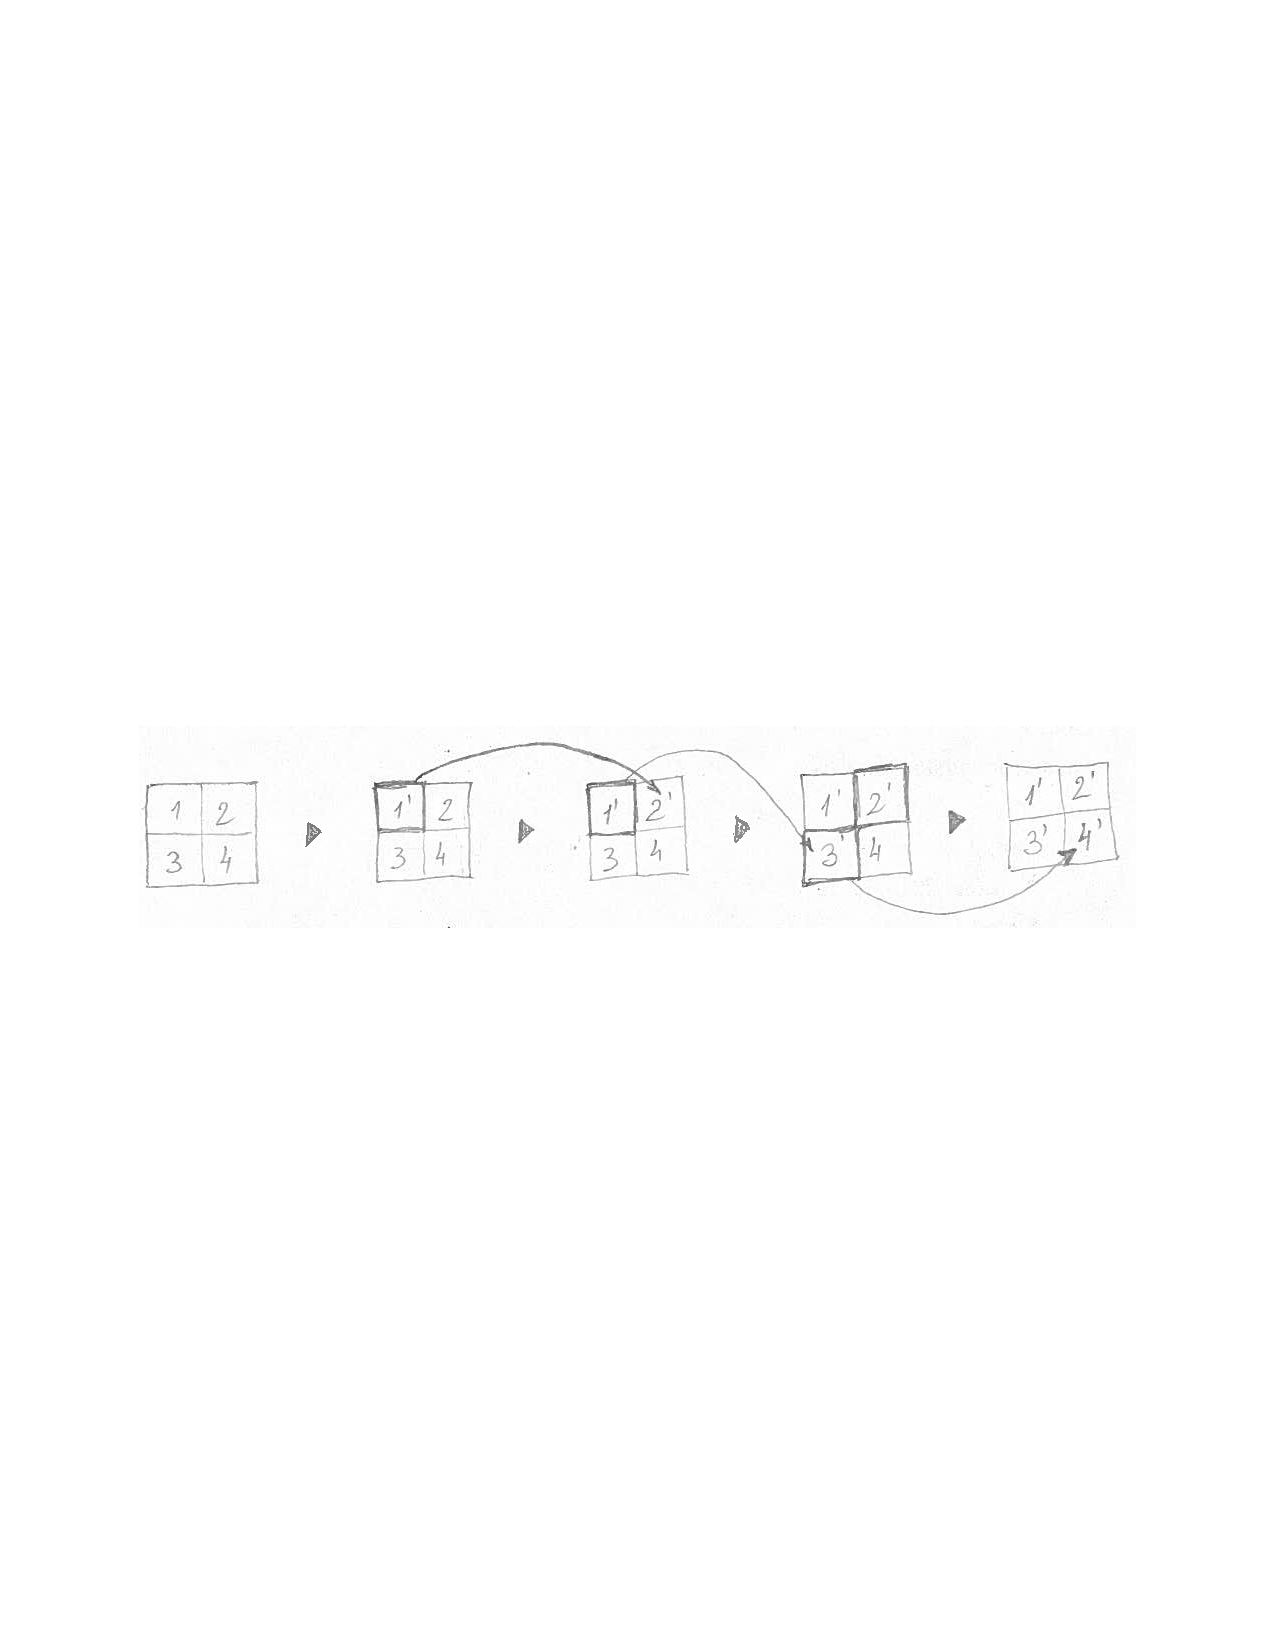
\includegraphics[width=.47\textwidth]{img/gap-stratify1}
\caption[caption]{\label{intro:chain}
  Stratified computation for Simplified Gap. \\[.2em]
  Thick borders indicate the region that is read at each step.}
\end{figure}

At this point it can be noticed that step 1 is equivalent to the original
algorithm when given as input the prefixes of $x$ and $y$ whose length correspond to the
height and width of \qbox1.

With the other three steps, however, things are not so simple:
each of them is required to process some data in addition to the input.
For example, step 2 is required to read values from \qbox1, due to the expression
$G_{iq}$ (where $\scriptstyle 0\leq q<j$).
In order to reason more formally, we define $J$ and $K$ the index sets of the rows
and columns, respectively; $J_0$, $J_1$ for the top and bottom row indexes, respectively;
and $K_0$, $K_1$ for the left and right column indexes (\Cref{intro:slice G}).
The specifications for step 2 then take the following form:

\begin{figure}
\[
\renewcommand\arraystretch{2}
\begin{array}{c|c|c|c|}
  \multicolumn{2}{c}{} & \multicolumn{2}{c}{K} \\ \cline{3-4}
  \multicolumn{2}{c}{} & \multicolumn{1}{c}{K_0}  & \multicolumn{1}{c}{K_1}\\ \cline{3-4}
  \multirow{2}{*}{$J$} & J_0 & 1 & 2 \\ \cline{3-4}
    & J_1 & 3 & 4 \\ \cline{3-4}
\end{array}
\]
\caption{\label{intro:slice G}
  Addressing quadrants in a two-dimensional array.}
\end{figure}

\makeatletter
\newcommand{\LeftEqNo}{\let\veqno\@@leqno}
\makeatother

\begin{equation}\LeftEqNo
\renewcommand\arraystretch{1.5}
\begin{array}{l@{}l}
	G_{\,(i :: J_0)\,(j :: K_1)} ~=~  \\
	\qquad
	\begin{cases}
		0                        & i=j=0 \\
		w_{0j}                   & i=0, j>0 \\
		w'_{i0}                  & i>0, j=0 \\
		\begin{array}{@{}l@{~}l}
		  \min\langle & \underset{0\leq (q::K) <j}\min ~ G_{iq} + w_{qj}, \\
		              & \underset{0\leq (p::J_0) <i}\min ~ G_{pj} + w'_{pi}~\rangle
		\end{array}              & i,j>0
	\end{cases}
\end{array}
\end{equation}

\medskip
Type annotations have been placed on $i$, $j$, $p$, and $q$ to define the regions
over which they range. $i::J_0, j::K_1$ means that the element $G_{ij}$
is always in \qbox2. Similarly, $G_{pj}$ is also in \qbox2. $G_{iq}$ is either in
\qbox1 or in \qbox2.

\begin{figure}
\begin{tabular}{l}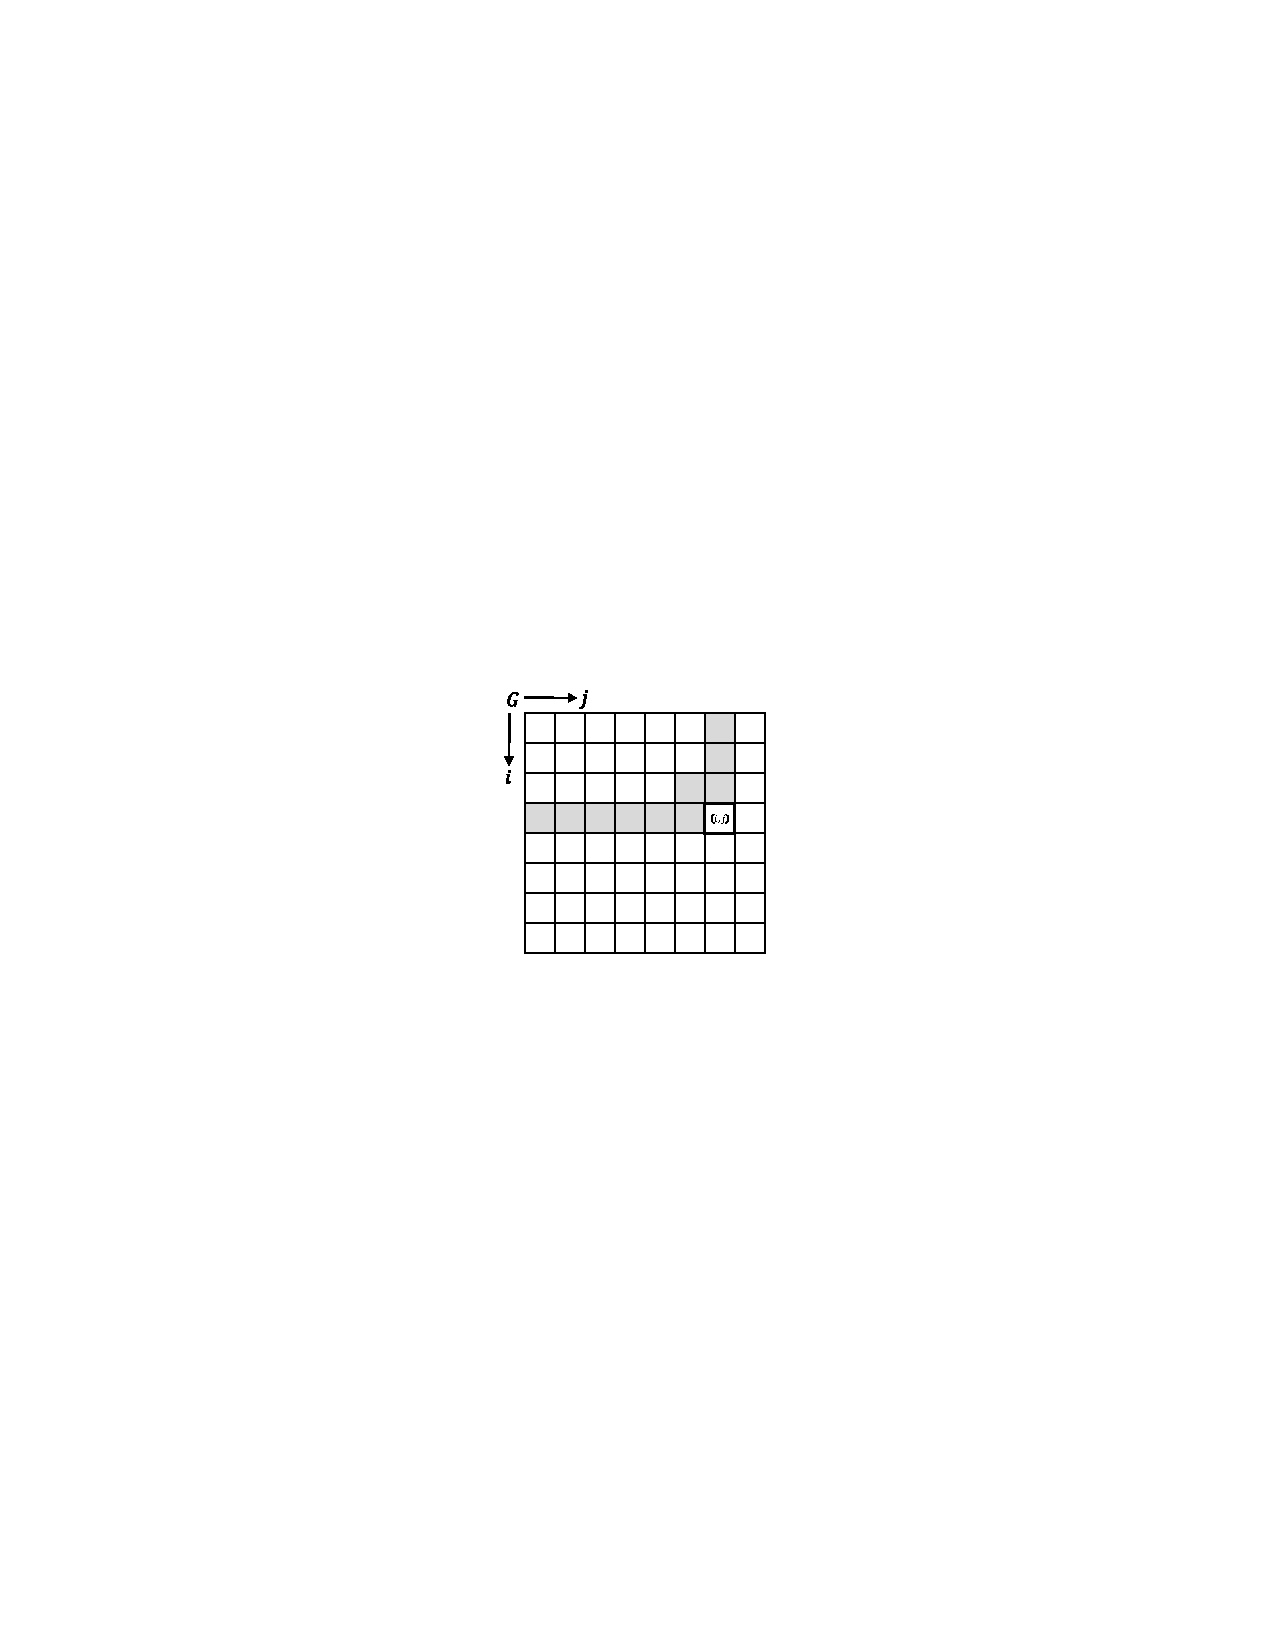
\includegraphics{img/gap-depend}\end{tabular}
\todo{for the simplified version, the cell (i-1,j-1) should not be grayed}
\caption{\label{intro:gap dependency matrix}}
\end{figure}

To address the situation, the algorithm designer would like to separate the parts
of the computation that read from \qbox1 from the parts that read from \qbox2.
This can be achieved here by splitting the $\min_{0\leq(q::K)<j}$ into two
ranges, according to the region in which $G_iq$ resides.

\begin{equation}\LeftEqNo
\renewcommand\arraystretch{1.5}
\begin{array}{l@{}l}
	G_{\,(i :: J_0)\,(j :: K_1)} ~=~  \\
	\qquad
	\begin{cases}
		0                        & i=j=0 \\
		w_{0j}                   & i=0, j>0 \\
		w'_{i0}                  & i>0, j=0 \\
		\begin{array}{@{}l@{~}l}
		  \min\langle & \underset{(q::K_0)}\min ~ G_{iq} + w_{qj}, \\
		              & \underset{(q::K_1) <j}\min ~ G_{iq} + w_{qj}, \\
		              & \underset{0\leq (p::J_0) <i}\min ~ G_{pj} + w'_{pi}~\rangle
		\end{array}              & i,j>0
	\end{cases}
\end{array}
\end{equation}

The path becomes clear: compute $\min_{(q::K_0)} ~ G_{iq} + w_{qj}$ first, for all $i$, $j$
in \qbox2. Then use the results to compute $G_{ij}$.

\begin{equation}\LeftEqNo
\renewcommand\arraystretch{1.5}
\begin{array}{l@{}l}
	G_{\,(i :: J_0)\,(j :: K_1)} ~=~  \\
	\qquad
	\textrm{let}~\psi_{ij} = \underset{(q::K_0)}\min ~ G_{iq} + w_{qj} \\
	\qquad\textrm{in} \\
	\qquad
	\begin{cases}
		0                        & i=j=0 \\
		w_{0j}                   & i=0, j>0 \\
		w'_{i0}                  & i>0, j=0 \\
		\begin{array}{@{}l@{~}l}
		  \min\langle & \psi_{ij}, \\
		              & \underset{(q::K_1) <j}\min ~ G_{iq} + w_{qj}, \\
		              & \underset{0\leq (p::J_0) <i}\min ~ G_{pj} + w'_{pi}~\rangle
		\end{array}              & i,j>0
	\end{cases}
\end{array}
\label{intro:let in 2}
\end{equation}

\medskip
The second part in \eqref{intro:let in 2} starts to look similar to \eqref{intro:gap spec}:
in particular, the types of $p$ and $q$ are the same as those of $i$ and $j$.
In fact, if we set $\psi_{ij}=\infty$, we get \eqref{intro:gap spec} as a special case,
only with $J_0$ and $K_1$ instead of $J$ and $K$.
It therefore makes sense to write a version that generalizes both.

\begin{equation}\LeftEqNo
\renewcommand\arraystretch{1.5}
\begin{array}{l}
	A_{\,\psi\, (i :: J)\, (j :: K)} ~=~  \\
	\qquad
	\begin{cases}
		0                        & i=j=0 \\
		w_{0j}                   & i=0, j>0 \\
		w'_{i0}                  & i>0, j=0 \\
		\begin{array}{@{}l@{~}l}
		  \min\langle & \psi_{ij}, \\
		              & \underset{(q::K)<j}\min ~ A_{\psi iq} + w_{qj}, \\
		              & \underset{(p::J)<i}\min ~ A_{\psi pj} + w'_{pi}~\rangle
		\end{array}              & i,j>0
	\end{cases}
\end{array}
\label{intro:gap phase A}
\end{equation}

\medskip
And we can now rewrite \eqref{intro:gap spec} and \eqref{intro:let in 2} as
%
\begin{equation}
	G_{ij} ~=~ A_{\,(\infty^{JK})\,(i::J)\,(j::K)}
\end{equation}
%
\begin{equation}
\renewcommand\arraystretch{1.3}
\begin{array}{l@{}l}
	G_{\,(i :: J_0)\,(j :: K_1)} ~=~ 
	& \textrm{let}~\psi_{ij} = \underset{(q::K_0)}\min ~ G_{iq} + w_{qj} \\
	& \textrm{in}~A_{\,\psi\,(i::J_0)\,(j::K_1)}
\end{array}	
\label{intro:let in 2 using A}
\end{equation}

\medskip
It takes a bit more insight to notice that \eqref{intro:let in 2 using A} can be further
generalized into:
%
\begin{equation}
\renewcommand\arraystretch{1.5}
\begin{array}{l@{}l}
	A_{\,\psi\,(i :: J)\,(j :: K)} ~=~  \qquad\mbox{(if $i\in J_0$, $j\in K_1$)}\\
	\qquad
	\textrm{let}~\psi'_{ij} = \min \langle~\psi_{ij}, \underset{(q::K_0)}\min ~ G_{iq} + w_{qj}~\rangle \\
	\qquad\textrm{in}~
	A_{\,\psi'\,(i::J_0)\,(j::K_1)}
\end{array}
\label{intro:let in A}
\end{equation}

That is the core of the divide and conquer method: representing the output as a combination
of smaller instances of the problem, or sub-problems, yielding a solution that is essentially
a recursive routine, or a set of mutually recursive routines. In \eqref{intro:let in A}, the
``let''-expression $\psi'_{ij} = \min \langle~\psi_{ij}, \min_{(q::K_0)} ~ G_{iq} + w_{qj}~\rangle$
is another sub-problem that has to be addressed using the same slicing technique.
Once all the pieces fit together, it is possible to cut the space into arbitrarily small pieces,
that fit nicely in each core's local cache. This greately increases performance, as demonstrated
by~\citneeded{perhaps include a table with exact figures}. 

\begin{center}$\vdots$
\end{center}

\subsection{Main Contributions}

\begin{enumerate}
  \item We develop a small set of tactics that can be used to transform a class of recurrence
  specifications intro equivalent divide-and-conquer programs, that admit parallel cache-local
  implementations, in a principled, systematic manner.
  \item We prove that these tactics are semantics-preserving, assuming some side conditions are met
  at the point when the tactic is applied.
  \item We show that the side conditions can be effectively translated into first-order closed
  formulas, and verified automatically by SMT solvers.
\end{enumerate}


\section{Overview}
\label{overview}

Most readers are likely familiar with the Dynamic Programming (DP) technique of Richard Bellman~\cite{03/Bellman:DP} to construct an optimal solution to a problem by combining together optimal solutions to many overlapping sub-problems. The key to DP is to exploit the overlap in order to explore otherwise exponential-sized problem spaces in polynomial time. Dynamic programs are usually described through recurrence relations that specify how the cells in a DP table must be filled using solutions already computed for other cells, but recent research has shown that it is possible to achieve order-of-magnitude performance improvements over this standard implementation approach by developing \emph{divide-and-conquer}  implementation strategies that recursively
partition the space of subproblems into smaller subspaces (see, e.g., \cite{IPDPS15/Tithi}).   For example, Tithi \etal{} have shown that for classical DP problems such as Floyd-Warshall, the parallel divide-and-conquer implementation is  8x faster  across a range of problem sizes compared with a parallel tiled implementation thanks to the better temporal locality and the additional optimization opportunities exposed by partitioning~\cite{IPDPS15/Tithi}. These performance differences matter because  DP is central to many important domains ranging from logistics to computational biology; as an illustrative example, a recent textbook \cite{DurbinEdKr98} on biological sequence analysis lists 11 applications of DP in bioinformatics just in its introductory chapter, with many more in chapters that follow. 

\newcommand{\xidx}{i}
\newcommand{\yidx}{j}
\newcommand{\xw}[1]{w^x_{#1}}
\newcommand{\yw}[1]{w^y_{#1}}

%To set up the premises, we are going to explain how an algorithms expert---we will call him Richard---would go about designing such an implementation by hand.
%We will then show how he will be able to do it more easily using Bellmania.

To illustrate the key concepts undelying Bellmania, we will walk through the first
few steps that an algorithms expert --- whom we will call Richard --- would follow to
generate a provably correct divide-and-conquer implementation of a DP algorithm.
As a motivating example, we consider the Simplified Arbiter problem.
Two processes $x$ and $y$ must be scheduled to run $n$ and $m$ seconds,
respectively, on a single processor, using one-second slots.
Execution starts at $t=0$. The cost for scheduling the slots $[a..b)$ of $x$ after
having scheduled slots $[0..c)$ of $y$
is given by $\xw{abc}$, and the cost for schedulting the slots $[a..b)$ of $y$
after scheduling $[0..c)$ of $x$ is given by $\yw{abc}$.

\begin{figure}[b]
\begin{tabular}{@{\hspace{-1pt}}r@{~}l@{}}
\begin{tikzpicture}[x=4.1mm,y=4.1mm,baseline=(center), remember picture]
  \coordinate(center) at (3,3);
  \draw[step=1] (0,0) grid (6,6);
  \draw[ultra thick] (4,2) rectangle +(1,1);
  %\node(Gij) at (4.5,2.5) {\tiny $\scriptscriptstyle\langle i,j\rangle$};
  \node[circle,fill=BrickRed,inner sep=0,minimum size=1mm](Gij) at (4.5,2.5) {};
  \fill[black,opacity=0.1] (0,5) rectangle (6,6);
  \fill[black,opacity=0.1] (0,0) rectangle (1,5);
  \fill[blue,opacity=0.2] (0,2) rectangle (4,3);
  \fill[blue,opacity=0.2] (4,3) rectangle (5,6);
  \node[anchor=south east](G) at (0,6) {\small$G$};
  \draw[->] (G.east) -- +(1.5,0) node[anchor=west] {\small $j$};
  \draw[->] (G.south) -- +(0,-1.5) node[anchor=north] {\small $i$};
\end{tikzpicture}
&
\small
$
\begin{array}{l@{}}
	\tikz[overlay, remember picture]{\draw[BrickRed] (0,0) -- (Gij);}
	G_{ij} ~=~ \\
	~
	\begin{cases}
		0                        & i=j=0 \\
		\yw{0j0}                  & i=0, j>0 \\
		\xw{0i0}                 & i>0, j=0 \\
		\begin{array}{@{}l@{\hspace{-1pt}}l@{\hspace{-4pt}}}
		  \min\langle & \underset{0\leq q<j}\min ~ G_{iq} + \yw{qji},  \\
		              & \underset{0\leq p<i}\min ~ G_{pj} + \xw{pij}~\rangle
		\end{array}              & i,j>0
	\end{cases}
\end{array}
$
\end{tabular}
\vspace{5pt}
\caption{Recurrence equation and cell-level dependencies.}
\label{overview:arbiter spec}
\end{figure}


The optimal cost for scheduling the first $i$ slots of $x$ and the first $j$ slots
of $y$ is given by the recurrence $G_{ij}$ in \Cref{overview:arbiter spec}. When $i$ is zero, it means that
only $y$ has been scheduled, so the cost is $\yw{0j0}$, and similarly when $j$ is zero, 
the cost is $\xw{0i0}$. When $i$ and $j$ are both positive, there are two options:
either the schedule ends with an allocation to $x$, 
where slots $[p..i)$ of $x$ were scheduled at $t=p+j$, and the cost is 
$G_{pj} + \xw{pij}$; or it ends with an allocation to $y$, where
slots $[q..j)$ of $y$ were scheduled at $t=i+q$, and the cost is $G_{iq} + \yw{qji}$.
The minimum over all respective $p<i$ and $q<j$ is taken.
Eventually, the optimal cost of the entire schedule is given by $G_{nm}$.

\begin{paragraph}{Iterative Algorithm.}
Using a standard dynamic programming method, our algorithm expert Richard would compute this recurrence
with an iterative program by understanding the dependency pattern:
to compute the $\min\langle\cdots\rangle$ expression in \Cref{overview:arbiter spec} and find the optimal
values for $p$ and $q$, the algorithm needs information from all cells above and to the left of $G_{ij}$.
In particular, each value $G_{ij}$ is computed from other values $G_{i'j'}$ with lower
indexes, $i'<i$, ~$j'<j$. 
Therefore, considering $G$ as a two-dimensional array, it can be filled in a single pass from left to right and from top
to bottom, as shown in \Cref{overview:iterative}.
\end{paragraph}

\newcommand\FORLINE[1]{\State\algorithmicfor~{#1} \algorithmicdo~}
\newcommand\Head[1]{\Comment{ {\it #1} ~~}}

\begin{algorithm}
\renewcommand\arraystretch{1.3}
\begin{algorithmic}
  \State $G_{00} := 0$    \Head{Initialize}
  \FORLINE{$i=1..n$}  $G_{i0} := \xw{0i0}$
  \FORLINE{$j=1..m$}  $G_{0j} := \yw{0j0}$  
  \For{$i=1..n$}          \Head{Compute}
    \For{$j=1..m$}
      \State $G_{ij} :=
        \begin{array}[t]{@{}l@{~}l} 
          \min\langle & \underset{0\leq q<j}\min ~ G_{iq} + \yw{qji}, \\
                      & \underset{0\leq p<i}\min ~ G_{pj} + \xw{pij}~\rangle \\         
        \end{array}$
    \EndFor
  \EndFor
\end{algorithmic}
\caption{\label{overview:iterative}
   Iterative Simplified Arbiter}
\end{algorithm}



\newcommand\qbox[1]{\fbox{\rm\scriptsize#1}}
\newcommand\tinyqbox[1]{\hspace{.5pt}\tikz \node[draw,inner sep=1.5pt] {$\scriptscriptstyle #1$};}

\newcommand\plusoneocd{\raisebox{.5pt}{$\scriptstyle+1$}}

\algrenewtext{Procedure}{\hspace{-3mm}{\bf procedure}~}  % hach to make proc header slighly less indented

\begin{paragraph}{Divide-and-Conquer Algorithm.}

\begin{figure}
\centering
\begin{tabular}{c@{\hspace{.5in}}c}
\begin{tikzpicture}[baseline=(n/2), q/.style={font=\relsize{1.3}}]
  \draw (0,0) grid (2,2);
  \node[q] at (.5,1.5) {1};   \node[q] at (1.5,1.5) {2};
  \node[q] at (.5, .5) {3};   \node[q] at (1.5, .5) {4};
  \node(O)[above left] at (0,2) {$0$};
  \node(m/2)[above] at (1,2) {$\frac{m}{2}$};
  \node(m)[above] at (2,2) {$m$};
  \node(n/2)[left] at (0,1) {$\frac{n}{2}$};
  \node(n)[left] at (0,0) {$n$};
  \node(J0)[above] at (.5,2.5) {$J_0$};
  \node(J1)[above] at (1.5,2.5) {$J_1$};
  \node(I0)[left] at (-.5,.5) {$I_0$};
  \node(I1)[left] at (-.5,1.5) {$I_1$};
  %\coordinate(0) at (0,0);
  %\coordinate(sw) at (0,0);
  %\coordinate(ne) at (2,2);
  %\draw (J0.north -| sw) -- node[above] {$J$} ++(ne |- 0);
  %\draw (I0.west |- sw) -- node[left] {$I$} ++(ne -| 0);
  \draw (O.north east) -- (O.north east -| m/2.north west);
  \draw (O.north east -| m.110) -- (O.north east -| m/2.north east);
  \draw (O.south west) -- (O.south west |- n/2.north west);
  \draw (O.south west |- n.160) -- (O.south west |- n/2.220);
\end{tikzpicture}
& 
$\begin{array}{l}\qbox1 \rightsquigarrow \qbox2 \\ 
\qbox1 \rightsquigarrow \qbox3 \\ \qbox2\rightsquigarrow \qbox4 \\ \qbox3 \rightsquigarrow \qbox4\end{array}$
\end{tabular}
\vspace{5pt}
\caption{\label{overview:quadrants}
  Dividing a two-dimensional array into quadrants; the dependencies are shown on the right.}
\end{figure}

Divide-and-conquer is a common algorithm development pattern (\cite{09/CLRS}, chapter 4) that has recently
been applied to DP (\cite{SODA06/Chowdhury,SPAA08/Chowdhury,TOCS10/Chowdhury,TCBB10/Chowdhury}).
This approach has the benefit of yielding cache-oblivious implementations by
increasing memory locality while preserving parallelism. With divide-and-conquer,
the DP table is partitioned into regions, and each region is expressed as a sub-problem
to be solved.

We will now describe how Richard approaches the running example using Bellmania.
He would like to partition the two-di\-men\-sio\-nal array $G$ into
quadrants, as illustrated in \Cref{overview:quadrants}.
In Bellmania, this is accomplished by applying the {\sf Slice} tactic,
illustrated graphically at the top of \Cref{overview:slice-stratify-synth}.
{\em Tactics} are transformation steps that manipulate the program,
and represent a high-level refinement concept.
The partitions are labeled $I_0,I_1$ and $J_0,J_1$ for row index ranges and column index ranges,
respectively.
Slicing gives the analog of the specification in \Cref{overview:logical-slice-stratify}({\it i}).
The expression inside $\min\langle\cdots\rangle$ is shortened for space,
but it is the same as in \Cref{overview:iterative}.

Following the same reasoning as in the iterative case, computing \qbox1
does not depend on any of the other computations. Richard applies the
{\sf Stratify} tactic, which encodes exactly this intuition: it separates
an independent computation step as a separate loop.
This is equivalent to rewriting the specification as in \Cref{overview:logical-slice-stratify}({\it ii}):
the first computation is given a special name $G^{\tinyqbox1}$, then the following
computations read data either from $G^{\tinyqbox1}$ (when the indices are in \qbox1)
or from $G$ (otherwise), which is denoted by $G^{\tinyqbox1}\!/G$. The ``$/\,$'' operator
is part of the Bellmania language and will be defined formally in \Cref{lang}.
Bellmania checks the data dependencies and verifies that the transformation
is sound.

Repeating {\sf Stratify} would result in a four-step computation
as seen in \Cref{overview:chain}, from which Richard can obtain the program in \Cref{overview:breakdown}
(only the first two steps are shown; remaining steps are analogous).
This already gives some performance gain, since the compututations \qbox2 and \qbox3
can now run in parallel. However, this is not what Richard wants; so he
changes the development of this procedure, which he calls ``A'', to produce
a recursive divide-and-conquer algorithm.
\end{paragraph}


\begin{figure}
\[\renewcommand\arraystretch{1.3}
  \begin{array}{@{}l@{}}
    \textsf{Slice} \quad i:\langle I_0|I_1\rangle \quad j:\langle J_0|J_1\rangle \hfill (i)\\
    ~\forall i,j\in\qbox1.~ G_{ij} = \min \langle\cdots G_{iq} \cdots G_{pj} \cdots \rangle \\
    ~\forall i,j\in\qbox2.~ G_{ij} = \min \langle\cdots G_{iq} \cdots G_{pj} \cdots \rangle \\
    ~\forall i,j\in\qbox3.~ G_{ij} = \min \langle\cdots G_{iq} \cdots G_{pj} \cdots \rangle \\
    ~\forall i,j\in\qbox4.~ G_{ij} = \min \langle\cdots G_{iq} \cdots G_{pj} \cdots \rangle \\
    %
    \textsf{Stratify} ~ \qbox1 \hfill (ii)\\
    %
    ~\forall i,j\in\qbox1.~ G^{\tinyqbox1}_{ij} = \min \langle\cdots G^{\tinyqbox1}_{iq} \cdots G^{\tinyqbox1}_{pj} \cdots \rangle \\
    ~\forall i,j\in\qbox2.~ G_{ij} = \min \langle\cdots (G^{\tinyqbox1}\!/G)_{iq} \cdots (G/G^{\tinyqbox1})_{pj} \cdots \rangle \\
    ~\forall i,j\in\qbox3.~ G_{ij} = \min \langle\cdots (G/G^{\tinyqbox1})_{iq} \cdots (G/G^{\tinyqbox1})_{pj} \cdots \rangle \\
    ~\forall i,j\in\qbox4.~ G_{ij} = \min \langle\cdots (G/G^{\tinyqbox1})_{iq} \cdots (G/G^{\tinyqbox1})_{pj} \cdots \rangle
  \end{array}
\]
\caption{\label{overview:logical-slice-stratify}
  The first two steps in the development, represented as logical specifications.}
\end{figure}


\newcommand\steparrowwidth{3mm}
\newcommand\steparrow{
\includegraphics[width=\steparrowwidth]{img/arrow}}

\begin{figure}
\centering
\ifarmando
\bigskip(missing figure)\bigskip
\else
\begin{tikzpicture}[>=latex,x=6mm,y=6mm,
    every path/.style={step=1},
    every node/.style={inner sep=.5pt},
    init data/.style={pattern=horizontal lines, pattern color=green!50!black},
    block/.style={rectangle,draw,very thick,fill=Orange, fill opacity=0.2, inner sep=0}]
    
  \def\dx{1.75cm}
    
  \fill[init data] (0,2) -- ++(.2,0) -- (2,.2) -- (2,0);
  \draw (0,0) grid (2,2);
  \node(s)[block,fit={(0,1) (1,2)}] {};
  %\node(1) at (.5,1.5) {1};   \node(2) at (1.5,1.5) {2};
  %\node(3) at (.5,.5) {3};    \node(4) at (1.5,.5) {4};

  \node[inner sep=0] at (2.5,1) {\steparrow};

  \tikzset{xshift=\dx}
  
  \draw (0,0) grid (2,2);
  \node(1) at (.5,1.5) {1};   %\node(2) at (1.5,1.5) {2};
  %\node(3) at (.5,.5) {3};         \node(4) at (1.5,.5) {4};
  \draw (s.70) edge[->,out=20] (1);
  \node(s)[block,fit={(1,0) (2,1)}] {};
  \node[inner sep=0] at (2.5,1) {\steparrow};

  \tikzset{xshift=\dx}
  
  \draw (0,0) grid (2,2);
  \node(1) at (.5,1.5) {1};  %\node(2) at (1.5,1.5) {2};
                             \node(4) at (1.5,.5) {4};
  \draw (s.-70) edge[->,out=-20,in=-135] (4);
  \fill[block] (0,2) |- (.85,1) to[out=0,in=90] (1,.85) |- (2,0) |- (1.15,1) to[out=180,in=-90] (1,1.15) |- cycle;
  \coordinate(s) at (1.8,0);
  \node[inner sep=0] at (2.5,1) {\steparrow};

  \tikzset{xshift=\dx}
  
  \draw (0,0) grid (2,2);
  \node(1) at (.5,1.5) {1};   \node(2) at (1.5,1.5) {2};
                              \node(4) at (1.5,.5) {4};
  \draw (s.south) edge[->,out=-40,in=-130] (2.-120);
  \coordinate (s) at (.8,0);

\end{tikzpicture}

\fi
\caption[caption]{\label{overview:chain}
  Stratified computation for Simplified Arbiter. \\[.2em]
  The array is initially empty except for the hatched area that is
  filled by {\it Initialize}.
  Shaded areas indicate the region that is read at each step.
  The arrows point at the quadrant that is written to. }
\end{figure}

\newcommand\applytactic[1]{{\tt >} \sf #1}
\newcommand\applytacticnode[1]{\node[right,align=left] at (3,1) {\applytactic{#1}}}


\begin{algorithm}
\renewcommand\arraystretch{1.3}
\begin{algorithmic}
\Procedure{A{\larger{[}}$G${\larger{]}}}{}\EndProcedure
  \For{$i=1..\frac{n}{2}$}    \Head{Compute \qbox1}
    \For{$j=1..\frac{m}{2}$} 
      \State \hspace{-.5cm}$G_{ij} :=
        \begin{array}{@{}l@{~}l} 
          \min\langle & \underset{0\leq q<j}\min ~ G_{iq} + \yw{qji}, 
                        \underset{0\leq p<i}\min ~ G_{pj} + \xw{pij}~\rangle \\         
        \end{array}$
    \EndFor
  \EndFor
  \For{$i=1..\frac{n}{2}$}    \Head{Compute \qbox2}
    \For{$j=\frac{m}{2}\plusoneocd..m$}
      \State \hspace{-.5cm}$G_{ij} :=
        \begin{array}[t]{@{}l@{~}l} 
          \min\langle & \underset{0\leq q<j}\min ~ G_{iq} + \yw{qji}, 
                        \underset{0\leq p<i}\min ~ G_{pj} + \xw{pij}~\rangle \\         
        \end{array}$
    \EndFor
  \EndFor
  \State $\vdots$ \Head{Compute \qbox3}
\end{algorithmic}
\caption{\label{overview:breakdown}
   Simplified Arbiter --- Sliced and Stratified}
\end{algorithm}

\begin{algorithm}
\renewcommand\arraystretch{1.3}
\begin{algorithmic}
\Procedure{A{\larger{[}}$G${\larger{]}}}{}\EndProcedure
  \State A\big[$G_{(0..\frac{n}{2})(0..\frac{m}{2})}$\big] \Head{Compute \qbox1}
  \For{$i=1..\frac{n}{2}$}    \Head{Compute \qbox2}
    \For{$j=\frac{m}{2}\plusoneocd..m$}
      \State $G_{ij} :=
        \begin{array}[t]{@{}l@{~}l} 
          \min\langle & \underset{0\leq q<\frac{m}{2}}\min ~ G_{iq} + \yw{qji}~\rangle \\         
        \end{array}$
          \Comment{(left)}
    \EndFor
  \EndFor
  \For{$i=1..\frac{n}{2}$}
    \For{$j=\frac{m}{2}\plusoneocd..m$}
      \State $G_{ij} :=
        \begin{array}[t]{@{}l@{~}l} 
          \min\langle G_{ij}, & \underset{\frac{m}{2}\leq q<j}\min ~ G_{iq} + \yw{qji}, \\
                      & \underset{0\leq p<i}\min ~ G_{pj} + \xw{pij}~\rangle \\         
        \end{array}$
          \Comment{(right)}
    \EndFor
  \EndFor
  \State $\vdots$
\end{algorithmic}
\caption{\label{overview:further-breakdown}
   Simplified Arbiter --- Sliced Even More}
\end{algorithm}


\newbox\primebox
\setbox\primebox\hbox{$'$}
\newbox\doubleprimebox
\setbox\doubleprimebox\hbox{$''$}

\newcommand\primeocd[1]{\hspace{\wd\primebox}#1\usebox\primebox}
\newcommand\doubleprimeocd[1]{\hspace{\wd\doubleprimebox}#1\usebox\doubleprimebox}

\begin{figure}
\centering
\ifarmando
\bigskip(missing figure)\bigskip
\else
\begin{tikzpicture}[>=latex,x=6mm,y=6mm,
    every path/.style={step=1},
    every node/.style={inner sep=.5pt},
    init data/.style={pattern=north west lines, pattern color=green!50!black},
    block/.style={rectangle,draw,very thick,fill=Orange, fill opacity=0.2, inner sep=0},
    knob/.style={midway,draw,fill=white,midway,inner sep=1.25pt}]
    
  \def\dx{1.75cm}
  \def\dy{1.75cm}
  
  % -------------------------------------------------------

  \draw (0,0) rectangle (2,2);
  \node(s)[block,fit={(0,0) (2,2)}] {};
  \node[inner sep=3mm](0) at (1,1) {0};

  \node[inner sep=0] at (2.5,1) {\steparrow};

  \tikzset{xshift=\dx}

  \draw (0,0) rectangle (2,2);
  \node[inner sep=3mm](0) at (1,1) {0$'$};
  \draw (s.70) edge[->,out=20] (0);

  \applytacticnode{Slice ~~ $i : \langle I_0|I_1\rangle$ ~~ $j : \langle J_0|J_1\rangle$};

  \tikzset{yshift=-\dy,xshift=-\dx}
    
  % -------------------------------------------------------

  \draw (0,0) grid (2,2);
  \node(1) at (.5,1.5) {1};   \node(2) at (1.5,1.5) {2};
  \node(3) at (.5, .5) {3};   \node(4) at (1.5, .5) {4};
  \node(s)[block,fit={(0,0) (2,2)}] {};

  \node[inner sep=0] at (2.5,1) {\steparrow};

  \tikzset{xshift=\dx}

  \draw (0,0) grid (2,2);
  \node(1) at (.5,1.5) {\primeocd 1};   \node(2) at (1.5,1.5) {\primeocd 2};
  \node(3) at (.5, .5) {\primeocd 3};   \node(4) at (1.5, .5) {\primeocd 4};
  \draw (s.70) edge[->,out=20] (1);
  \draw (s.70) edge[->,out=20] (2);
  \draw (s.70) edge[->,out=20] (3);
  \draw (s.70) edge[->,out=20] (4);

  \applytacticnode{Stratify \qbox1};

  % -------------------------------------------------------
  \setlength\baselineskip{15pt}  

  \tikzset{yshift=-\dy,xshift=-\dx}

  \draw (0,0) grid (2,2);
  \node(s)[block,fit={(0,1) (1,2)}] {};
  \node(1) at (.5,1.5) {1};   \node(2) at (1.5,1.5) {2};
  \node(3) at (.5, .5) {3};   \node(4) at (1.5, .5) {4};

  \node[inner sep=0] at (2.5,1) {\steparrow};

  \tikzset{xshift=\dx}
  
  \draw (0,0) grid (2,2);
  \node(1) at (.5,1.5) {\primeocd 1};   \node(2) at (1.5,1.5) {2};
  \node(3) at (.5, .5) {3};             \node(4) at (1.5,.5) {4};
  \draw (s.70) edge[->,out=20] node[knob,circle] {} (1);
  \node(s)[block,fit={(0,0) (2,2)}] {};
  
  \node[inner sep=0] at (2.5,1) {\steparrow};

  \tikzset{xshift=\dx}

  \draw (0,0) grid (2,2);
  \node(1) at (.5,1.5) {\primeocd 1};   \node(2) at (1.5,1.5) {\primeocd 2};
  \node(3) at (.5, .5) {\primeocd 3};   \node(4) at (1.5, .5) {\primeocd 4};
  \draw (s.70) edge[->,out=20] (2);
  \draw (s.70) edge[->,out=20] (3);
  \draw (s.70) edge[->,out=20] (4);
  
  \applytacticnode{Synth $\circ ~~ \dashrightarrow A^{I_0J_0}$ \\ 
      \applytactic{Stratify \qbox2}};
  
  \tikzset{yshift=-\dy,xshift=-2*\dx}

  % -------------------------------------------------------

  \draw (0,0) grid (2,2);
  \node(s)[block,fit={(0,1) (1,2)}] {};
  \node(1) at (.5,1.5) {1};   \node(2) at (1.5,1.5) {2};
  \node(3) at (.5, .5) {3};   \node(4) at (1.5, .5) {4};

  \node[inner sep=0] at (2.5,1) {\steparrow};

  \tikzset{xshift=\dx}
  
  \draw (0,0) grid (2,2);
  \node(1) at (.5,1.5) {\primeocd 1};   \node(2) at (1.5,1.5) {2};
  \node(3) at (.5, .5) {3};   \node(4) at (1.5, .5) {4};
  \draw (s.70) edge[->,out=20] node[knob,circle] {} (1);
  \node(s)[block,fit={(0,1) (2,2)}] {};
  \node[inner sep=0] at (2.5,1) {\steparrow};

  \tikzset{xshift=\dx}
  
  \draw (0,0) grid (2,2);
  \node(1) at (.5,1.5) {\primeocd 1};  \node(2) at (1.5,1.5) {\primeocd 2};
  \node(3) at (.5,.5) {3};             \node(4) at (1.5,.5) {4};
  \draw (s.70) edge[->,out=20] (2);
  \node[inner sep=0] at (2.8,1) {$\cdots$};

  \tikzset{xshift=.25*\dx}

  \node[right,align=left] at (3,1) {\applytactic{Slice \qbox2 \\ \quad $p : \langle J_0|J_1\rangle$}};

  \tikzset{yshift=-\dy,xshift=-2.25*\dx}

  % -------------------------------------------------------

  \draw (0,0) grid (2,2);
  \node(s)[block,fit={(0,1) (1,2)}] {};
  \node(1) at (.5,1.5) {1};   \node(2) at (1.5,1.5) {2};
  \node(3) at (.5, .5) {3};   \node(4) at (1.5, .5) {4};

  \node[inner sep=0] at (2.5,1) {\steparrow};

  \tikzset{xshift=\dx}
  
  \draw (0,0) grid (2,2);
  \node(1) at (.5,1.5) {\primeocd 1};   \node(2) at (1.5,1.5) {2};
  \node(3) at (.5, .5) {3};   \node(4) at (1.5, .5) {4};
  \draw (s.70) edge[->,out=20] node[knob,circle] {} (1);
  \node(s1)[block,fit={(0,1) (1,2)}] {};
  \node(s2)[block,fit={(1,1) (2,2)}] {};
  
  \node[inner sep=0] at (2.5,1) {\steparrow};

  \tikzset{xshift=\dx}
  
  \draw (0,0) grid (2,2);
  \node(1) at (.5,1.5) {\primeocd 1};  \node(2) at (1.5,1.5) {\primeocd 2};
  \node(3) at (.5,.5) {3};             \node(4) at (1.5,.5) {4};
  \draw (s1.70) edge[->,out=20] (2);
  \draw (s2.70) edge[->,out=20] (2);
  \node[inner sep=0] at (2.8,1) {$\cdots$};

  \tikzset{xshift=.25*\dx}

  \node[right,align=left] at (3,1) {\applytactic{Stratify \qbox2$^{\# 1}$}};

  \tikzset{yshift=-\dy,xshift=-2.25*\dx}

  % -------------------------------------------------------

  \draw (0,0) grid (2,2);
  \node(s)[block,fit={(0,1) (1,2)}] {};
  \node(1) at (.5,1.5) {1};   \node(2) at (1.5,1.5) {2};
  \node(3) at (.5, .5) {3};   \node(4) at (1.5, .5) {4};

  \node[inner sep=0] at (2.5,1) {\steparrow};

  \tikzset{xshift=\dx}
  
  \draw (0,0) grid (2,2);
  \node(1) at (.5,1.5) {\primeocd 1};   \node(2) at (1.5,1.5) {2};
  \node(3) at (.5, .5) {3};   \node(4) at (1.5, .5) {4};
  \draw (s.70) edge[->,out=20] node[knob,circle] {} (1);
  \node(s)[block,fit={(0,1) (1,2)}] {};
  
  \node[inner sep=0] at (2.5,1) {\steparrow};

  \tikzset{xshift=\dx}
  
  \draw (0,0) grid (2,2);
  \node(1) at (.5,1.5) {\primeocd 1};  \node(2) at (1.5,1.5) {\primeocd 2};
  \node(3) at (.5,.5) {3};             \node(4) at (1.5,.5) {4};
  \draw (s.70) edge[->,out=20] node[knob,isosceles triangle,rotate=90] {} (2);
  \node(s)[block,fit={(1,1) (2,2)}] {};

  \node[inner sep=0] at (2.5,1) {\steparrow};

  \tikzset{xshift=\dx}
  
  \draw (0,0) grid (2,2);
  \node(1) at (.5,1.5) {\primeocd 1};  \node(2) at (1.5,1.5) {\doubleprimeocd 2};
  \node(3) at (.5,.5) {3};             \node(4) at (1.5,.5) {4};
  \draw (s.70) edge[->,out=20] node[knob,diamond] {} (2);
  \node[inner sep=0] at (2.8,1) {$\cdots$};

  \tikzset{xshift=-1.25*\dx,yshift=-.75*\dy}

  \applytacticnode{Synth {\tikz\node[knob,isosceles triangle,rotate=90] {};} $~~ \longrightarrow B^{I_0J_0J_1}$ \\ 
      \applytactic{Synth $\diamond$} $~~ \dashrightarrow A^{I_0J_1}$};

  \tikzset{yshift=-\dy,xshift=-2*\dx}

\end{tikzpicture}

\vspace{-2mm}
\fi
\caption[caption]{\label{overview:slice-stratify-synth}
  Overview of tactic semantics in Bellmania. }
\end{figure}


\medskip
At this point, Richard notices that {\it Compute \qbox1} is just a smaller version of
the original {\it Compute}; so following {\sf Stratify} \qbox1, he invokes {\sf Synth}, which automatically
synthesizes a recursive call A\big[$G_{(0..\frac{n}{2})(0..\frac{m}{2})}$\big]
(presented using abstract index ranges as $A^{I_0J_0}$).

The other steps require some further algebraic manipulation.
Observe that the computation of \qbox2 is {\bf not} equivalent to
A\big[$G_{(0..\frac{n}{2})(\frac{m}{2}..m)}$], 
because when $\frac{m}{2} \leq j < m$, the range $0\leq q < j$ leads to
some accesses $G_{iq}$ lying outside of \qbox2.

Richard addressed this problem by splitting the range of $q$ using the {\sf Slice}
tactic again, effectively breaking the original $\min\langle\cdots\rangle$ into two:
one where $0\leq q < \frac{m}{2}$,
and one where $\frac{m}{2}\leq q < j$. 
He uses {\sf Stratify} to organize the loops in the program such that both 
loops write to the same area, namely \qbox2, where the second loop reads data
written by the first loop, as shown in \Cref{overview:further-breakdown}.
It is important to notice that the first loop only reads from \qbox1, 
while the second loop only reads from \qbox2.

The computation of \qbox2:(right) is now a true copy of A,
with sub-matrix $G_{(0..\frac{n}{2})(\frac{m}{2}..m)}$ (with the small caveat,
that A has to be changed to include the term $G_{ij}$ in the $\min\langle~\rangle$ expression).
Again, Bellmania synthesizes the sub-call and proves the equivalence.
Running {\sf Synth} on \qbox2:(left) will reveal that it is a new computation,
to which Richard gives the name ``B''. 

After repeating
the same reasoning steps to \qbox3 and \qbox4,
Richard finally has the version in \Cref{overview:recursive-A}.
The base case (when $G$ is small) is added automatically by the Bellmania compiler.
The specific size bound needs to be tuned for performance.\footnote{The auto-tuning step is not implemented in the current version.}


\begin{algorithm}
\renewcommand\arraystretch{1.3}
\begin{algorithmic}
\Procedure{A{\larger{[}}$G${\larger{]}}}{}\EndProcedure
  \If{$G$ {\it is very small}} {\it run iterative version}
  \Else
  \State A\big[$G_{(0..\frac{n}{2})(0..\frac{m}{2})}$\big] \Head{Compute \qbox1}
  \State B\big[$G_{(0..\frac{n}{2})(0..\frac{m}{2})}, 
                G_{(0..\frac{n}{2})(\frac{m}{2}..m)}$\big]    \Head{Compute \qbox2}
  \State A\big[$G_{(0..\frac{n}{2})(\frac{m}{2}..m)}$\big]
  \State C\big[$G_{(0..\frac{n}{2})(0..\frac{m}{2})}, 
                G_{(\frac{n}{2}..n)(0..\frac{m}{2})}$\big]    \Head{Compute \qbox3}
  \State A\big[$G_{(\frac{n}{2}..n)(0..\frac{m}{2})}$\big]
  \State B\big[$G_{(\frac{n}{2}..n)(0..\frac{m}{2})}, 
                G_{(\frac{n}{2}..n)(\frac{m}{2}..m)}$\big]    \Head{Compute \qbox4}
  \State C\big[$G_{(0..\frac{n}{2})(\frac{m}{2}..m)}, 
                G_{(\frac{n}{2}..n)(\frac{m}{2}..m)}$\big]
  \State A\big[$G_{(0..\frac{n}{2})(\frac{m}{2}..m)}$\big]
  \EndIf
\end{algorithmic}
\caption{\label{overview:recursive-A}
   Simplified Arbiter --- Recursive Version}
\end{algorithm}

Richard must then use the same strategy to further break down and
transform the computations of B and C, each into four recursive sub-computations, 
further improving the locality of the resulting algorithm.
Eventually, through these transformations, he can succeed in breaking the computation of $G$ into recursive sub-computations leading to a true divide-and-conquer algorithm. 

As is well illustrated by the example, this line of reasoning can get quite complicated for most dynamic programming algorithms, 
and producing a correct divide-and-conquer algorithm for a given dynamic programming problem is considered quite difficult even by the researchers who originally pioneered the technique. 
Fortunately, the reasoning can be mechanized in Bellmania, which allows
Richard and other algorithm designers to produce an implementation of this algorithm
as well as a {\bf machine-checked proof} of correctness
through a series of high-level tactic application.

Overall, it took Richard only about 10 steps to construct \Cref{overview:recursive-A},
and a total of 26 steps to construct all three steps of the Simplified Arbiter,
comprising an implementation that is 10$\times$ faster than a parallel
\Cref{overview:iterative} generated by a state-of-the-art parallelizing compiler.
The user is greatly assisted by tactics like {\sf Synth}, that carry out the monotonic
and error-prone task of choosing the right parameters for each recursive call; also,
mistakes are identified early in the development thanks to automatic verification,
saving hours of debugging later on.

Once a divide-and-conquer algorithm is found, generating an optimal implementation still requires some additional work, such as finding the right point at which to switch to an iterative algorithm to leverage SIMD parallelism as well as low-level tuning and compiler optimization;
these steps are performed by more traditional compiler optimization techniques
as discussed in \Cref{codegen}.

In the following sections, we describe the different components of Bellmania. 
The system utilizes \newterm{solver-aided tactics} to manipulate a given specification
and generate provably correct pseudo-code; 
this approach is demonstrated by engineering specialized tactics for the domain of divide-and-conquer DP.

\section{A Unified Language}

\newcommand\semp[1]{[\![{#1}]\!]}
\newcommand\fix{\operatorname{fix}}

We first set up a formal language that we will use to describe computations and reason about them.
Bellmania uses the same language for specifications and for programs.  Its core is the polymorphic
$\lambda$-calculus, that is, simply typed $\lambda$-calculus with universally quantified type variables 
(also known as \newterm{System F}).

We write abstraction terms as $(v:\T)\mapsto e$, where $\T$ is the type of the argument $v$ and $e$ is
the body. Curried functions $(v_1:\T_1)\mapsto (v_2:\T_2) \mapsto \cdots \mapsto (v_n:\T_n) \mapsto e$ are abbreviated 
as $(v_1:\T_1)\cdots(v_n:\T_n)\mapsto e$.

The semantics differ slightly from that of traditional functional languages: arrow types $\T_1\to\T_2$
are interpreted as {\bf mappings} from values of type $\T_1$ to values of type $\T_2$. Algebraically,
interpretations of types, $\semp{\T_1}$, $\semp{\T_2}$, are sets, and interpretations of arrow-typed terms,
$f : \T_1\to\T_2$, are {\bf partial functions} --- $\semp{f} : \semp{\T_1}\rightharpoonup\semp{\T_2}$.
This implies that a term $t : \T$ may evaluate to an \newterm{undefined} value, $\semp{t}=\bot_\T$
(We would shorten it to $\semp{t}=\bot$ when the type is either insignificant or understood from the context).
For simplicity, we shall identify $\bot_{\T_1\to\T_2}$ with the empty mapping $(v:\T_1)\mapsto\bot_{\T_2}$.

All functions are naturally extended, so that $f\,\bot=\bot$.

\subsection{Operators}
\label{lang:operators}

The core is augmented with the following intrinsic operators:

\begin{itemize}
  \item A fixed point operator $\fix f$, with the denotational semantics
    \[\semp{\fix f} ~=~ \sigma x.~ (\semp f\,x=x)\]
  we assume that recurrences given in specifications are well-defined, 
  such that $\semp f$ has a single fixed point.
  In other words, we ignore nonterminating computations.
  \item A guard operator $[\,]_{_\square}\,$, which comes in two flavors:
  \[\begin{array}{l}
      [x]_{\mathit{cond}} = \begin{cases}x & \mathit{cond} \\ \bot & \lnot\mathit{cond}\end{cases} \\
      {}[f]_{P_1\times P_2\times \cdots P_n} = \overline{x} \mapsto [f\,\overline{x}]_{\bigwedge P_i(x_i)}
    \end{array}\]
  where $\overline{x} = x_1 \cdots x_n$. This second form can be used to
  refer to quadrants of an array; for example, in \Cref{overview:quadrants-abstract}, $\qbox2 \equiv G\big|_{J_0\times J_1}$.
  \item A slash operator $/$,     \vspace{-2pt}
  \[\renewcommand\arraystretch{1.5}
    \begin{array}{ll}
      \mbox{For scalars $x,y:\S$} & x/y = \begin{cases}x & \mbox{if }x\neq\bot \\ y & \mbox{if }x=\bot\end{cases} \\
      \mbox{For $f,g:\T_1\to\T_2$} & f/g = (v:\T_1)\mapsto (f\,v)/(g\,v)
    \end{array}\]
  This operator is typically used to combine computations done on
  parts of the array. For example, \[\psi\mapsto \big[f\,\psi\big]_{I_0} ~ \Big/ ~ \big[g\,\psi\big]_{I_1}\]
  combines a result of $f$ in the lower indices of a (one-dimensional) array
  with a result of $g$ in the higher indices ($I_0$ and $I_1$, respectively, are the index subsets).
  In our concrete syntax, $\big|$ take precedence over $/$,
  and function application takes precedence over both.
  Notice that this does not limit the areas from which $f$ and $g$ read,
  and they are free to access the entire domain of $\psi$.
\end{itemize}

\subsection{Types and Type Qualifiers}

We extend the type system with predicate abstraction in the form of logically qualified data types 
(Liquid Types~\cite{PLDI08/Rondon}). These are refinement types restricted via a set of abstraction predicates,
called \newterm{qualifiers}, which are defined over the base types.
Contradictory to the general use of refinement types, the purpose of these qualifiers is not to
check a program for safety and reject ill-typed program, but rather to serve as annotations for
tactics, to convey information to the solver for use in the proof, and later to help the compiler
to properly schedule parallel computations.

More specifically, typing $f : \{v:\T_1 \,|\, P(v)\}\to\T_2$ would mean that $f\,x$
can only be defined where $P(x)$ is true; otherwise, $f\,x=\bot$. 
It {\bf does not} mean that $x$ has to have the qualifier $P$ at compile time for the term $f\,x$
to be well-typed.

As such, we define a Bellmania program to be well-typed iff it is well-typed
without the annotations (in its \newterm{raw form}). Qualifiers are processed
as a separate pass to properly annotate sub-terms.

Some qualifiers are built-in, and more can defined by the user. To keep the syntax simple, we somewhat
limit the use of qualifiers, allowing only the following forms:

\begin{itemize}
  \item $\{v:\T ~|~ P(v)\}$, abbreviated as $\T\cap P$. When the signature of $P$ is known (which is
  almost always), it is enough to write $P$.
  \item $\{v:\T ~|~ P(v)\land Q(v)\}$, abbreviated as $\T\cap P\cap Q$, or just $P\cap Q$. This extends
  to any number of conjuncts of the same form.
  \item $(x : \T_2) \to \{v:\T_2 ~|~ R(x,v)\} \to \T_3$, abbreviated as $\big((\T_1\times\T_2)\cap R\big)\to\T_3$.
  The qualifier argument $x$ must be the preceding argument; this extends to predicates of
  any arity (that is, a $k$-ary predicate in a qualifier is applied to the $k$
  arguments to the left of it, including the one where it appears).
\end{itemize}


\medskip  
The type refinement operators $\cap$ and $\times$ may be composed to create \newterm{droplets},
using the abstract syntax in \Cref{lang:droplets}.
Note that the language does not define tuple types; hence there is no distinction between curried and uncurried function types.
Droplets can express conjunctions of qualifiers,
as long as their argument sets are either disjoint or contained, but not overlapping;
for example, \[x:\{v:\T_1~|~P(v)\}\to \{v:\T_2~|~Q(v)\land R(x,v)\}\to\T_3\] can be written as
$\big((P\times Q)\cap R\big)\to\T_3$, but \[x:\T_1\to y:\{v:\T_2~|~R(x,v)\} \to \{v:\T_3~|~R(y,v)\}\to\T_4\]
cannot be represented as a droplet.

As with any refinement type system, we define the \newterm{shape} of a droplet to be the raw type
obtained from it by removing all qualifiers.

\newcommand\examplePar{%
\noindent\hspace{-2pt}%
\tikz[baseline=(E.base)]\node(E)[draw,rectangle,rounded corners=.7em] {\bf Example};
}
\examplePar
The inputs $\xw{}$, $\yw{}$ to the Simplified Arbiter (\Cref{intro:arbiter spec}) can be typed using these droplets:
\[
\begin{array}{l}
  \xw{} : ((I\times I)\cap{<})\to J\to\R \\
  \yw{} : ((J\times J)\cap{<})\to I\to\R
\end{array}
\]

This states that $w\,p\,i\,j$ is only defined for $p<i$. It doesn't {\em force} it to be defined,
as it is still a partial function. This property is in fact useful: we now have a mechanism for
specifying that some schedules are impossible, by setting the respective $w\,p\,i\,j=\bot$!

\subsubsection*{Typing Rules}

\begin{figure}
\[
\begin{array}{lcll}
  d       & ::= & e^1 \quad |\quad e^k\to d \\
  e^1     & ::= & \T & \mbox{\it\small for scalar type $\T$} \\
  e^{k+l} & ::= & e^k \times e^l \\
  e^k     & ::= & e^k \cap P & \mbox{\it\small for $k$-ary predicate symbol $P$} 
\end{array}
\]
\caption{\label{lang:droplets}
  Syntax of type qualifiers (droplets). $k$, $l$ are positive integer
  dimension indexes.}
\end{figure}

As mentioned earlier, annotations are ignored when typechecking a term.
This gives a simple characteristic of type safety without the need to
explictly write any new typing rules. It also means that for $f:\T_1\to\T_2$, $x:T_3$, we obtain $f\,x:\T_2$ whenever
$\T_1$ and $\T_3$ have the same shape. This requires some explanation.

Considering a (partial) function $\T\to\S$ to be a set of pairs of elements $\langle x,y\rangle$ 
from its domain $\T$ and range $\S$, respectively, it is clear to see that any function of type $\T_1\to\S_1$,
such that $\semp{\T_1}\subseteq\semp{\T}$, $\semp{\S_1}\subseteq\semp{\S}$, 
is \emph{also}, by definition, a function of type $\T\to\S$, since $\semp{\T_1}\times\semp{\S_1}\subseteq\semp{\T}\times\semp{\S}$.
If we define subtyping as inclusion of the domains, i.e. $\T_1 <:\T$ whenever $\semp{\T_1}\subseteq\semp{\T}$,
this translates into:
%
\[\T_1<:\T ~\land~ \S_1<:\S ~~\Rightarrow~~ (\T_1\to\S_1) <: (\T\to\S)\]

In this case, the type constructor $\to$ is {\bf covariant} in both arguments.\footnote{This is different from classical view, and holds in this case because we interpret functions as \emph{mappings}.}
With this in mind, a function $g:(\T\to\S)\to \S_2$ can be called with an argument $a: \T_1\to\S_1$,
by regular subtyping rules, and $g\,a : \S_2$.

When the argument's type is not a subtype, but has the same shape as that of the expected type,
it is \newterm{coerced} to the required type by restricting the values to the desired proper subset.
%
\[\mbox{For }h:\T\to\S \qquad \semp{h\,a} ~=~ \semp{h}\big(\semp{a} :: \T\big)\]

Where $::$ is defined as follows:
\begin{itemize}
  \item For scalar (non-arrow) type $\T$, \[x :: \T ~=~ \begin{cases}x & \mbox{if }x\in\semp{\T} \\ \bot & \mbox{if }x\not\in\semp{\T}\end{cases}\]
  \item $f :: \T\to\S ~=~ x\mapsto \big(f\,(x :: \T)\big) :: \S$
\end{itemize}

\medskip
We extend our abstract syntax with an explicit \newterm{cast operator}
$t::\T$ following this semantics.

\subsubsection*{Type Inference}

Base types are inferred normally as in a classical Hindley-Milner type system.
The operators (\Cref{lang:operators}) behave like polymorphic
constants with the following types:
\[\renewcommand\arraystretch{1.5}
  \begin{array}{c}
    {\fix} : (\T\to\T)\to\T \qquad {/} : \T\to\T\to\T \\
    (::\T) : \mathrm{shape}[\T]\to\mathrm{shape}[\T]
  \end{array}\]


Qualifiers are also inferred by essentially propagating them up and down the syntax tree.
Since the program already typechecks once the base types are in place, the problem is no longer
one of finding {\em valid} annotations, but rather of {\em tightening} them as much as possible
without introducing semantics-changing coercions. For example, $(f :: I\to(I\cap P))\,i$ may
be assigned the type $I$, but it can also be assigned $I\cap P$ without changing its semantics.

Qualifiers are propagated by defining a \newterm{type intersection} operator $\sqcap$ that
takes two droplets of the same shape $\T_1$, $\T_2$ and returns a droplet with a conjunction of all the qualifiers
occuring in either $\T_1$ or $\T_2$. The operator is defined in terms of the corresponding liquid types:
\begin{itemize}
  \item If $\T_1=\{v:\T ~|~ \varphi_1\}$ and $\T_2=\{v:\T ~|~ \varphi_2\}$,
	\[\T_1\sqcap\T_2 ~=~ \{v:\T ~|~ \varphi_1\land\varphi_2\}\]
  \item If $\T_1=x:\S_1\to\S_2$, $\T_2=x:\S_3\to\S_4$ (named arguments are normalized so that $\T_1$ and $\T_2$ use the same names),
    \[\T_1\sqcap\T_2 ~=~ x:(\S_1\sqcap\S_3)\to(\S_2\sqcap\S_4)\]
\end{itemize}

We then define the \newterm{type refinement} steps for $e$ a sub-term, listed in \Cref{lang:type refinement rules}.
These rules are applied continuously until a fixed point is reached.
The resulting types are eventually converted back to droplet form (expressed via $\cap$ and $\times$);
qualifiers that cannot be expressed in droplets are discarded.

\begin{figure*}
\newcommand\typerule[2]{{\renewcommand\arraystretch{1.5}\begin{array}[t]{c} #1 \\ \hline #2 \end{array}}}
\[
\renewcommand\arraystretch{4}
\begin{array}{cccp{1cm}}
  \multirow{2}{1cm}[-3em]{\begin{tikzpicture}\draw (1mm,6em) -- (0,6em) -- (0,-5em) node[midway,above,xshift=-2mm,rotate=90] {Core language} -- +(1mm,0);\end{tikzpicture}} &
  \typerule{e=v \qquad \Gamma,v:\T_1\vdash e:\T_0}
           {\Gamma,v:\T_1 ~\vdash~ e:\T_0\sqcap\T_1} &
  \typerule{e=e_1\,e_2 \qquad \Gamma \vdash e:\T, ~ e_1:\T_1, ~ e_2:\T_2\to\S_2}
           {\renewcommand\arraystretch{1.2}
            \begin{array}[t]{@{}l@{}l@{}}
              \Gamma ~\vdash~ & e:\T\sqcap\S_2, \\ 
                              & e_1:\T_1\sqcap\T_2, \\
                              & e_2:(\T_1\to\T)\sqcap(\T_2\to\S_2)
            \end{array}} & \\
  &
  \cspan2{
  \typerule{e=(v:\T)\mapsto e_1 \qquad \Gamma\vdash e:\T_0\to\S_0 \qquad \Gamma,v:\T\sqcap\T_0\vdash e_1:\T_1}
           {\renewcommand\arraystretch{1.2}
            \begin{array}[t]{r@{}l}
              \Gamma ~\vdash~ & e:(\T_0\to\S_0)\sqcap(\T\to\T_1)\\
              \Gamma,v:\T\sqcap\T_0 ~\vdash~ & e_1:\T_1\sqcap\S_0 
            \end{array}}  } & \\
  %
  \multirow{2}{1cm}[-2.5em]{\begin{tikzpicture}\draw (1mm,0) -- (0,0) -- (0,-8em) node[midway,above,xshift=-2mm,rotate=90] {Extensions} -- +(1mm,0);\end{tikzpicture}} &
  \typerule{e=\fix e_1 \qquad \Gamma\vdash e:\T, ~ e_1:\T_1\to\T_2}          % fix
           {\Gamma\vdash e: \T\sqcap\T_2} &
  \typerule{e=e_1/e_2 \qquad \Gamma\vdash e:\T, ~ e_1:\T_1, ~ e_2:\T_2}      % /
           {\renewcommand\arraystretch{1.2}
            \begin{array}[t]{@{}l@{}l@{}}
              \Gamma\vdash{} & e_1:\T_1\sqcap\T \\ & 
                               e_2:\T_2\sqcap\T
            \end{array}} & \\
  &
  \cspan2{
  \typerule{e=e_1::\T \qquad \Gamma\vdash e_1:\T_1}                           % ::
           {\Gamma\vdash e:\T\sqcap\T_1, ~ e_1:\T\sqcap\T_1} } &
\end{array}
\]
\caption{\label{lang:type refinement rules}
  Type refinement rules, for inferring qualifiers in sub-expressions.}
\end{figure*}

Note that two syntactically identical terms in different sub-trees may be assigned
different types by this method. This is a desirable property, as (some) context information
gets encoded in the type that way.

\examplePar Let $I_0\subseteq I$ be a unary predicate, and $0:T$ a constant.
The expression $f\,(i:I_0)\mapsto f\,i\,i ~/~ 0$ will induce the following type
inferences:

\hspace*{\fill}
\begin{tikzpicture}[node distance=1em]
  \node(farg) {$f$};
  \node(iarg)[right=of farg] {$(i:I_0)$};
  \node(mapsto)[right=of iarg] {$\mapsto$};
  \node(f)[right=of mapsto] {$f$};
  \node(i1)[right=of f] {$i$};
  \node(i2)[right=of i1] {$i$};
  \node(slash)[right=of i2] {$\big/$};
  \node(zero)[right=of slash] {$0$};
  \node(l0)[coordinate,below=1mm of farg] {};
  \node(l1)[coordinate,below=4.5mm of l0] {};
  \node(l2)[coordinate,below=3.5mm of l1] {};
  \node(l3)[coordinate,below=3.5mm of l2] {};
  \node(l4)[coordinate,below=3.5mm of l3] {};
  \def\ytip{2pt}
  \draw (l0 -| farg.west) -- +(0,-\ytip) -| (l0 -| farg.east) node[pos=0.25,below] {\tiny $I\to I\to T$};
  \draw (l0 -| f.west) -- +(0,-\ytip) -| (l0 -| f.east) node[pos=0.5,anchor=north east,inner xsep=0] {\tiny $I_0\to I_0\to T$};
  \draw (l0 -| i1.west) -- +(0,-\ytip) -| (l0 -| i1.east) node[pos=0.25,below] {\tiny $I_0$};
  \draw (l0 -| i2.west) -- +(0,-\ytip) -| (l0 -| i2.east) node[pos=0.25,below] {\tiny $I_0$};
  \draw (l0 -| zero.west) -- +(0,-\ytip) -| (l0 -| zero.east) node[pos=0.25,below] {\tiny $T$};
  \draw (l1 -| f.west) -- +(0,-\ytip) -| (l1 -| i1.east) node[pos=0.25,below] {\tiny $I_0\to T$};
  \draw (l2 -| f.west) -- +(0,-\ytip) -| (l2 -| i2.east) node[pos=0.25,below] {\tiny $T$};
  \draw (l3 -| f.west) -- +(0,-\ytip) -| (l3 -| zero.east) node[pos=0.25,below] {\tiny $T$};
  \draw (l4 -| farg.west) -- +(0,-\ytip) -| (l4 -| zero.east) node[pos=0.25,below] {\tiny $(I\to I\to T)\to I_0\to T$};
\end{tikzpicture}
\hspace*{\fill}

\subsection{Primitives}

The standard library contains some common primitives:

\begin{itemize}
  \item $\R$, a type for real numbers; $\N$ for natural numbers; $\B$ for Boolean true/false.
  \item ${=} : \T\to\T\to\B$, always interpreted as equality.
  \item ${+}, {-} : \T\to\T\to\T$, polymorphic binary operators.
  \item ${<} : \T\to\T\to\B$, a polymorphic order relation.
  \item $cons : \T\to(\N\to\T)\to(\N\to\T), nil : \N\to\T$, list constructors.
  \item $\min, \max, \Sigma : (\T\to\S)\to\S$, reduction (aggregation) operators
    on ordered/unordered collections. The collection is represented by a mapping $f : \T\to\S$,
    so that e.g. \[\semp{\min f} = \min \big\{\semp{f}\,v \;\big|\; v\in\semp{\T}, \semp{f}\,v\neq\bot\big\}\]
    The collections are expected to be finite.
\end{itemize}

\subsection{Additional Notation}
\newcommand\applt{\textrm{{\scriptsize\,}\guillemotright{\scriptsize\,}}}

We also adopt some syntactic sugar to make complex terms more managable:

\begin{itemize}
  \item $x \applt f ~=~ f\,x$ for application from the left.
  \item $\langle t_1,\cdots,t_n\rangle = cons t_1 (cons \cdots (cons t_n nil) \cdots)$
    for fixed-length lists.
\end{itemize}


\exampleTitle  \begin{comment}\subsection{Example}\end{comment}

\noindent
The specification of the Simplified Gap (\Cref{intro:arbiter spec}) will be written as
%
\begin{equation}
  \renewcommand\arraystretch{1.5}
  \begin{array}{@{}l@{}l@{}l@{}}
    \lspan3{\xw : ((I\times I)\cap{<})\to J\to\R} \\
    \lspan3{\yw : ((J\times J)\cap{<})\to I\to\R} \\
    G ~=~ \fix \theta\,i\,j\mapsto{}
      & \lspan2{\big[0\big]_{i=j=0} \,\Big/~ \big[\yw{0j0}\big]_{i=0} \,\Big/~ \big[\xw{0i0}\big]_{j=0} \,\Big/} \\
      & \min~\langle~ & \min p\mapsto\theta_{pj}+\xw{pij}, \\
      & & \min q\mapsto\theta_{iq}+\yw{qji} ~\rangle
  \end{array}
  \label{lang:arbiter spec}
\end{equation}

\medskip
We are using $f_{xy}$
as a more readable alternative typography for $f\,x\,y$,
where $f$ is a function symbol and $x$, $y$ are its arguments.

Note that the ranges for $\min p$ and $\min q$ are implicit, from the types of
$\xw{}$, $\yw{}$: \[\xw{pij}\neq\bot\limplies p<i \quad \mbox{and} \quad \yw{qji}\neq\bot\limplies q<j\]

\medskip
\hrule

\section{Tactics}
\label{tactics}

We now define the method by which that our framework transforms program terms, by means of \newterm{tactics}.
A tactic is a scheme of equalities that can be used for rewriting.
When applied to a program term, any occurrence of the {\bf left-hand side} is replaced by the {\bf right-hand side}.%
\footnote{This is also a standard convention in Coq, for example.}
A valid application of a tactic is an instance of the scheme that is well-typed and logically valid
(that is, the two sides have the same interpretation in any structure that interprets the free
variables occurring in the equality).

The application of tactics yields a sequence of program terms, each of which is checked to
be equivalent to the previous one. We refer to this sequence by the name \newterm{development}.

We associate with each tactic some \newterm{proof obligations}, listed after the word \textbf{\textit{Obligations}}
in the following paragraph.
When applying a tactic instance, these obligations are also instantiated and given to an automated prover. 
If verified successfully, they entail the validity of the instance. 
Clearly the tactic itself can be used as its proof obligation, if it is easy enough to prove automatically; 
in such cases we write ``\textbf{\textit{Obligations}:} tactic.''

The following are the major tactics provided by our framework. 
More tactic definitions are given in the appendix.

\newcommand\Obligations{\medskip\noindent\textbf{\textit{Obligations}:} }
\newcommand\reduce{\operatorname{reduce}}
\newcommand\listConcat{{\scriptstyle \,++\,}}

\theoremstyle{definition}
\newtheorem{tactic}{Tactic}

\newcommand\tacticdef[1]{\subsection*{\sf\larger #1}\vspace{-3mm}}
\newcommand\tacticdefcompact[1]{\medskip\noindent{\sf\larger #1}\medskip\hfill}

\tacticdefcompact{Slice} \label{tactics:Slice}
$f ~=~ \big[f\big]_{X_1} ~\Big/~ \big[f\big]_{X_2} ~\Big/ ~\cdots~ \Big/~ \big[f\big]_{X_r}$\hspace{10mm}

This tactic partitions a mapping into sub-regions. Each $X_i$ may be a cross product ($\times$)
according to the arity of $f$.

\Obligations tactic.

Informally, the recombination expression is equal to $f$
when $X_{1..r}$ ``cover'' all the defined points of $f$ (also known as the \newterm{support} of $f$).

\medskip
\tacticdefcompact{Stratify}
$\fix (f\applt g) ~=~ (\fix f) ~\applt~ \big(\psi\mapsto \fix (\widehat\psi\applt g)\big)$
\\
where $\widehat\psi$ abbreviates $\theta\mapsto\psi$, with fresh variable $\theta$.

This tactic is used to break a long (recursive) computation into simpler sub-computations.
$\psi$ may be fresh, or it may reuse a variable already occurring in $g$, rebinding those occurrences.
An example is required to understand why this is useful.

Let $h=\theta\mapsto\big([t_0]_{I_0}\big/[t_1]_{I_1}\big)$, where $t_{0,1}$ are terms with free variable $\theta$.
Stratification is done by setting $f=\theta\mapsto t_0$ and
 $g=f\,\theta\mapsto [f\,\theta]_{I_0}\big/[t_1]_{I_1}$. We get $\fix h=\fix(f\applt g)$; {\sf~Stratify}
breaks it into $\fix f$ and $\psi\mapsto \fix (\widehat\psi\applt g)$,
which get simplified with $\beta$-reduction, giving the expression the form:

\vspace{-5mm}
\[\big(\fix(\theta\mapsto t_0)\big) ~\applt~ 
  \Big(\psi\mapsto \fix \big(\theta\mapsto[\psi]_{I_0}\big/[t_1]_{I_1}\big)\Big)\]

\vspace{-2mm}
This precisely encodes our intuition of computing the fixed point of $t_0$ first,
then $t_1$ based on the result of $t_0$.

\Obligations Let $h=f\applt g$ and $g'=\psi\mapsto\widehat\psi\applt g$. Let $\theta,\zeta$ be
fresh variables.
\begin{equation}
\renewcommand\arraystretch{1.5}
\begin{array}{l@{\qquad}l}
f\,(g'\,\zeta\,\theta) ~=~ f\,\zeta &
g'\,(f\,\theta)\,\theta ~=~ h\,\theta
\end{array}
\label{tactics:Stratify obligations}
\end{equation}

Proof is given in \Cref{tactics:soundness}.

\tacticdef{Synth} \label{tactics:Synth}
\[\fix\big(h_1 ~\big/~ \cdots ~\big/~ h_r\big) ~=~ 
  f_1 :: \T_1 ~\big/~ \cdots ~\big/~ f_r :: \T_r\]

This tactic is used to generate recursive calls to sub-programs. For $i=1..r$, $f_i$
is one of the following: $\fix h_i$, $h_i\,\psi$, or $t\,\psi$, where $\psi$ is some
variable and $t$ is a term corresponding to a previously defined subroutine
($A$, $B$, $C$ in the example).
Bellmania chooses these values automatically (see \Cref{tactics:synthesis}),
but the user may override it.

\newcommand\Y{\mathcal{Y}}

\Obligations Let $h=h_1/\cdots/h_r$, and let $\T\to\T$ be the shape of $h$. 
  For each $f_i$, depending on the form of $f_i$:
\begin{itemize}
  \item If $f_i \cong \fix f$ --- \\
    \rule{0pt}{12pt}
    $h :: (\T \to \Y) = h :: (\Y \to \Y) = g :: (\Y \to \T)$
    for some $\Y$ which is a subtype of $\T$ and a supertype of $\T_i$.
  \item If $f_i$ does not contain any ``$\fix$'' terms ---\\
    \rule{0pt}{12pt}
    $h\,(h\,\theta) :: \T_i = f_i :: \T_i$ for a fresh variable $\theta$.
\end{itemize}

We use $\cong$ to denote syntactic congruence up to $\beta$-reduction.

\begin{comment}
\Obligations Let $h=h_1/\cdots/h_r$, let $\overline\theta\!=\!\theta_{1..r}$ be $r$ fresh variables, and let
$f = \theta_{1..r} \mapsto (f_1\,\theta_1)::\T_1/\cdots/(f_r\,\theta_r)::\T_r$.
\begin{itemize}
  \item $\T_{1..r}$ are disjoint mappings.
  \item {\bf Either}\quad $h\,(f\,\overline\theta) = f\,\overline\theta$ \\{\bf or}\qquad
  $\begin{array}[t]{l} h\,\theta=\theta ~\limplies~ (f_i\,\theta :: \T_i)=\theta :: \T_i ~, \\
  \theta::\T_1~/~\cdots~/~\theta::\T_r=\theta\end{array}$
\end{itemize}

(We give two alternatives, as the first is usually easier to prove, but may hold in less cases)
\end{comment}


\newenvironment{tacticbox}[1]{\begin{center}
  \begin{tabular}{|@{~~~~}l@{~~~~}|}\hline
    \rule{0pt}{2.3ex}\underline{\sf \,#1\,}\\[.4em]$}
  {$\\[-1em] \\[.3ex] \hline \end{tabular} \end{center}}


\subsection{Synthesis-supported {\sf Synth} Tactic}
\label{tactics:synthesis}

As mentioned in \Cref{intro,overview}, the user is assisted by automatic
inference while applying tactics. In particular, the {\sf Synth} tactic requires
the user to specify a subroutine to call and parameters to call it with.
In addition, the subtype $\Y$ is required to complete the correctness proof.
To automate this task, Bellmania employs {\cegis}, a software synthesis technique
implemented in the tool {\Sketch}~\cite{STTT13/Solar-Lezama}. The proof obligations, along with the possible
space of parameter assignments taken from the set of sub-types defined during
{\sf Slice}, are translated to {\Sketch}. Since {\Sketch} uses bounded domains,
the result is then verified using full SMT.

While the size of the search space is not huge, typically in the order of \textasciitilde50
alternatives, it is usually hard for the user to figure out which exact call
should be made. Since {\sf Synth} is used extensively throughout the develoment,
This kind of automation greatly improves overall usability.

\subsection{Soundness}
\label{tactics:soundness}

\renewenvironment{proof}{\noindent{\bf Proof.~}}{}

\begin{theorem}
Let $s=s'$ be an instance of one of the tactics introduced in this section.
let $a_i=b_i$, $i=1..k$, be the proof obligations. If $\semp{a_i}=\semp{b_i}$
for all interpretations of the free variables of $a_i$ and $b_i$, then
$\semp{s}=\semp{s'}$ for all interpretations of the free variables of $s$ and $s'$.
\end{theorem}

\begin{proof}
For the tactics with \textbf{\textit{Obligations}:} tactic, the theorem is trivial.

\medskip
\noindent
{\tt >} For {\sf Stratify}, let $f$, $g$ be partial functions such that
\vspace{-.5em}
\[\renewcommand\arraystretch{1.3}
  \forall \theta,\zeta.\quad \begin{array}{l}f\,(g\,\zeta\,\theta) ~=~ f\,\zeta \quad\land\quad
  g\,(f\,\theta)\,\theta ~=~ h\,\theta
  \end{array}\quad\]
  
Assume that $\zeta = \fix f$ and $\theta = \fix (g\,\zeta)$. 
That is, $f\,\zeta = \zeta$ and $g\,\zeta\,\theta = \theta$.
Then ---
\vspace{-.5em}
\[\renewcommand\arraystretch{1.3}
  \begin{array}{l@{}l}
   h\,\theta & {}= g\,(f\,\theta)\,\theta = g\,(f\,(g\,\zeta\,\theta))\,\theta =
              g\,(f\,\zeta)\,\theta = \theta
  \end{array}\]
  
\noindent
So $\theta = \fix h$. We get $\fix h = \fix \big(g \,(\fix f)\big)$; equivalently,
\[\fix h = (\fix f) \applt \big(\psi\mapsto\fix (g\,\psi)\big)\]

Now instantiate $h$, $f$, and $g$, with $f\applt g$, $f$, and $g'$ from \Cref{tactics:Stratify obligations},
and we obtain the equality in the tactic.

\medskip
\noindent
{\tt >} For {\sf Synth}, ({\it i}) assume $f_i=\fix g$ and
\[h :: \T\to\Y = h :: \Y\to\Y = g :: \Y\to\T\]

Intuitively, $\Y$ ``cuts out'' a region of an array $\theta :: \T$ given
as input to $h$ and $g$. This area is self-contained, in the sense that
only elements in $\Y$ are needed to compute elements in $\Y$, as indicated
by the refined type $\Y\to\Y$.

Notice that from the premise follows $g :: \Y\to\T = g :: \Y\to\Y$. We use the following corollary:

\medskip\noindent
{\bf Corollary.~} Let $f : \T\to\T$; if either $f :: \T\to\Y = f :: \Y\to\Y$ or $f :: \Y\to\T = f :: \Y\to\Y$, 
then $(\fix f)::\Y = \fix (f :: \Y\to\Y)$.

Proof is included in the appendix.

\medskip
From the corollary, and for the given $h$ and $g$, we learn that $(\fix h)::\Y = \fix(h::\Y\to\Y)$,
and also $(\fix g)::\Y=\fix(g::\Y\to\Y)$. Since $h::\Y\to\Y=g::\Y\to\Y$,
we get $(\fix h)::\Y = (\fix g)::\Y$; now, $\Y$ is a supertype of $\T_i$, so $(\theta::\Y)::\T_i=\theta::\T_i$:
\[\renewcommand\arraystretch{1.3}
  \begin{array}{l}(\fix h)::\T_i = ((\fix h)::\Y)::\T_i = ((\fix g)::\Y)::\T_i = \\
    \qquad = (\fix g)::\T_i=f_i::\T_i
  \end{array}\]

{\it (ii)} Assume $h\,(h\,\theta) :: \T_i = f_i :: \T_i$ holds for any $\theta:\T$,
then in particlar, for $\theta=\fix\,h$, we get $h\,(h\,\fix h) :: \T_i = f_i :: \T_i$.
Since $h\,(h\,\fix h) = \fix h$, we obtain the conjecture $(\fix h) :: \T_i = f_i :: \T_i$.
\qed
\end{proof}

\medskip
Our reliance on the termination of $\fix$ expressions may seem conspicuous, since some of these
expressions are generated automatically by the system. However, a closer look reveals that whenever
such a computation is introduced, the set of the recursive calls is makes is a subset of those made by the existing one.
Therefore, if the original recurrence terminates, so does the new one. In any case, all the recurrences
in our development have a trivial termination argument (the indexes $i$,$j$ change monotonically between calls),
so practically, this should never become a problem.

\newcommand\vtyped[2]{\underset{\scriptscriptstyle ( #2 )}{ #1 }}


\section{Automating Proofs}

This section describes the encoding of proof obligations in (many-sorted) first-order logic,
and the ways in which type information is used in discharging them.

Each base type is associated with a sort. The qualifiers are naturally encoded
as predicate symbols with appropriate sorts. In the following paragraphs, we
use a type and its associated sort interchangeably, and the meaning should be clear
from the context.

Each free variable and each node in the formula syntax tree are assigned two
symbols: a function symbol representing the values, and a predicate symbol
representing the support, that is, the set of tuples for which there is a mapping.
For example, a variable $f : J\to\R$ will be assigned a function $f^1: J\to\R$
and a predicate $|f|: J\to\B$. The superscript indictes the function's arity,
and the vertical bars indicate the support.

For refinement-typed symbols, the first-order symbols are still defined in terms
of the shape, and an assumption concerning the support is emitted. For example,
for $g: (J\cap P)\to\R$, the symbols $g^1:J\to\R$, $|g|:J\to\B$ are defined,
with the assumption $\forall \alpha:J.~|g|(\alpha)\limplies P(\alpha)$.

Assumptions are similarly created for nodes of the syntax tree of the formula to
be verified. We define the \newterm{enclosure} of a node to be the ordered set of
all the variables bound by ancestor abstraction nodes ($v\mapsto\ldots$). Since
the interpretation of the node depends on the values of these variables, it is
``skolemized'', i.e., its type is prefixed by the types of enclosing variables.
For example, if $e:\T$, then inside a term $(v:\S)\mapsto \cdots e\cdots$ it would be treated as
type $\S\to\T$.

Typically, the goal is an equality between functions $f=g$. This naturally translates
to first-order logic as
\[\forall\overline{\alpha}.~\big(|f|(\overline\alpha)\liff|g|(\overline\alpha)\big) \land
  \big(|f|(\overline\alpha) \limplies f^k(\overline\alpha)=g^k(\overline\alpha)\big)\]

\begin{paragraph}{First-class functions.}
When a function is being used as an argument in an application term, 
we take its arrow type $\T\to\S$ and create a \newterm{faux sort} $F_{\T\to\S}$,
an ``apply'' operator $@ : F_{\T\to\S}\to\T\to\S$, and the \newterm{extensionality axiom} ---
\begin{equation}
\forall \alpha\alpha'.~ \big(\forall\beta.~ @(\alpha,\beta)=@(\alpha',\beta)\big)\limplies \alpha=\alpha'
\label{automated:extensionality}
\end{equation}

Then for each such function symbol $f^k:\T\to\S$ used as argument, we create its 
\newterm{reflection} $f^0:F_{\T\to\S}$ defined by
\begin{equation}
\forall \overline\alpha.~~@(f^0,\overline\alpha)=f^k(\overline\alpha)
\label{automated:reflection}
\end{equation}
\end{paragraph}

\subsection{Simplification}
\label{automated:simplification}

When $f$,$g$ of the goal $f=g$, are abstraction terms, the above can be simplified by
introducing $k$ fresh variables, $\overline x=x_1\cdots x_k$, and writing the goal as
$f\,\overline x = g\,\overline x$. The types of $\overline x$ are inferred from the types
of $f$ and $g$ (which should have the same shape). We can then apply $\beta$-reduction as
a simplification step. This dramatically reduces the number of quantifiers in the first-order
theory representing the goal, making SMT solving feasible.

Moreover, if the goal has the form $f\,t_1 = f\,t_2$ (e.g. {\sf Stratify}, \Cref{tactics}) it may
be worth trying to prove that $t_1::\T = t_2::\T$, where $f:\T\to\S$.
This trivially entails the goal and is (usually) much easier to prove. 

Another useful technique is common subexpression elimination, which is quite standard
in compiler optimizations. Tactic applications tend to create copies of terms, so
merging identical subexpressions into a single symbol can drastically reduce the size
of the SMT encoding.

\section{Code Generation}
\label{codegen}

We built a compiler for programs in Bellmania language that generates efficient C++ code parallelized with Intel Cilk constructs. The compiler uses type information from the development to improve the
quality of generated code. From the types of sub-terms corresponding
to array indices, the compiler extracts information about what region
of the array is read by each computation, and from the types of $\lambda$-bound index variable it constructs loops that write to
the appropriate regions. The compiler utilizes the SMT solver to infer dependency constraints as in~\cite{JACM67/Karp},
and figures out the direction of each loop (ascending or descending). 
In addition, inter-quadrant dependencies can be used to determine which computations can be run in parallel (at the granularity of
function calls) based on a fork-join model;
two calls are considered non-conflicting if each write region is disjoint from the others' read and write regions.
\cbstart\diffnote{explained the role of types in our static analysis}%
Type information is heavily utilized here: occurrences of array variables signify reads,
so their types denote (an over-approximation of) the region being ``read from'',
whereas return types denote the region being ``written to''.
Disjointness can be decided using propositional logic through the predicate abstraction induced by type qualifiers.
\cbend

The compiler also employs more traditional optimization techniques
to further simplify the code and improve its running time:
(1) lifts conditionals to loop bounds via simple interval analysis, %to optimize the loop bounds and performs some traditional compiler %transformations to reduce the number of iterations and comparisons,
(2) eliminates redundant iterations and comparisons that can be resolved at compile time,
(3) identifies loops that read non-contiguous memory blocks and applies copy optimization~\cite{ASPLOS91/Lam} automatically to better utilize caches. Examples of generated code are included in the supplemental material with this submission,
and
\cbstart
(4) follows a simple heuristic that inserts loop vectorization directives.
\cbend
 
%Use Cilk for parallelization - references later
%Using SMT solver and type information to find directions of loops for fixed point computations
%Using type information and SMT solvers to parallelize different components
%Using type information to optimize the loop bounds, reduce checking of guards and do copy optimization
%Traditional compiler transformations

%code can be found in repo
%JACM67: Recurrences to loops: http://dl.acm.org/citation.cfm?id=321418
%ASPLOS1991: copy optimization: http://suif.stanford.edu/papers/lam-asplos91.pdf
\section{Empirical Evaluation}

We implemented our technique and used it to generate cache-oblivious
divide-and-conquer implementations of three algorithms that were used as
benchmarks in \cite{IPDPS15/Tithi}, and a few others.

\begin{paragraph}{Gap problem.}
A generalized minimal edit distance problem. Given two input strings 
$\overline{x}=x_1\cdots x_m$ and $\overline{y}=y_1\cdots y_n$,
compute the cost of transforming $x$ into $y$ by any combination of the
following steps
\begin{itemize}
  \item Replacing $x_i$ with $y_j$, at cost $c_{ij}$.
  \item Deleting $x_{p+1}\cdots x_q$, at cost $\xw{pq}$.
  \item Inserting $y_{p+1}\cdots y_q$ in $\overline{x}$, at cost $\yw{pq}$.
\end{itemize}

The computation is given by the recurrence \Cref{evaluation:gap spec}.
\end{paragraph}

\begin{paragraph}{Parenthesis problem.} Compute
an optimal placements of parenthesis in a long chain of multiplication, e.g. of matrices, where the input is
are cost functions $x_i$ for accessing the $i$-th element and
$w_{ikj}$ for multiplying elements $[i,k)$ by elements $[k,j)$.
The corresponding recurrence is shown in \Cref{evaluation:paren spec}.
\end{paragraph}

\begin{paragraph}{Protein Accordion Folding problem.} A protein can be viewed
as a string $\mathcal{P}_{1..n}$ over an alphabet of amino acids. 
The protein folds itself in a way that minimizes potential energy.
Some of the acids are {\em hydrophobic}; minimization of the total hydrophobic
area exposed to water is a major driving force of the folding process.
One possible model is packing $\mathcal{P}$ in a two-dimensional square lattice
in a way that maximizes the number of pairs of hydrophobic elements,
where the shape of the fold is an {\em accordion}, alternating between going down and going
up.
\end{paragraph}

\medskip
We also exercised our system on a number of textbook problems:
the Longest Common Subsequence (LCS) problem, the Knapsack problem,
and the Bitonic Traveling Salesman problem.

\begin{figure}
\[
  \renewcommand\arraystretch{1.5}
  \begin{array}{@{}l@{}l@{}l@{}}
    \lspan3{\xw :: ((J\times J)\cap{<})\to\R} \\
    \lspan3{\yw :: ((K\times K)\cap{<})\to\R} \\
    G ~=~ \fix \theta\,i\,j\mapsto{}
      & \lspan2{\big[0\big]_{i=j=0} ~\Big/~ \big[\yw{0j}\big]_{i=0} ~\Big/~ \big[\xw{i0}\big]_{j=0} ~\Big/~} \\
      & \min~\langle~ & \theta_{(i-1)\,(j-1)} + c_{ij},\\
      & & \min p\mapsto\theta_{pj}+\xw{pi}, \\
      & & \min q\mapsto\theta_{iq}+\yw{qj} ~\rangle
  \end{array}
\]
\caption{\label{evaluation:gap spec}
  Specifications for the full version of the Gap DP problem.}
\end{figure}

\begin{figure}
\[
  \renewcommand\arraystretch{1.5}
  \begin{array}{@{}l@{}l}
    \lspan2{x :: J\to\R} \\
    \lspan2{w :: (J\times J\times J)\to\R} \\
    E ~=~ \fix \theta\,i\,j\mapsto{}
      & {\big[x_{ij}\big]_{i+1=j} ~\Big/~} \\
      & \min k\mapsto\theta_{ik}+\theta_{kj}+w_{ikj} \\
  \end{array}
\]
\caption{\label{evaluation:paren spec}
  Specifications for the Parenthesis Assignment DP problem.}
\end{figure}


The tactic application engine is implemented in Scala. We implemeted a prototype
IDE using HTML5 and AngularJS, which communicates with the engine by sending
and receiving program terms serialized as JSON. Our system supports using either
Z3 or CVC4 as the back-end SMT solver for discharging proof obligations required
for soundness proofs. The compiler for programs in Bellmania is implemented in 
python and generates C++ code with Intel Cilk constructs for parallelization.


Table~\ref{table:cppruns} shows the performance improvement for the auto-generated 
implementation (AUTO) as compared to the standard parallelized loop implementation 
(LOOPDP). The table also compares it with state-of-the-art parallelized 
implementations (CO and COZ). It can be seen from the table that our 
implementation performs close to the manually optimized code. 
Figure~\ref{fig:gap} depicts the performance of these implementations 
as a function of problem size and shows the scalability of our technique. %ROHIT:scalability of what:the technique or the code?



\begin{table}
\centering
\renewcommand\a{({\it i})}    % relax! it's only for this figure
\renewcommand\b{({\it ii})}
\renewcommand\c{({\it iii})}
\begin{tabular}{|l|r|rrr|r|}
  \cline{2-6}
  \multicolumn{1}{c|}{} &    & \multicolumn{4}{c|}{\small Average solving time ({\it s})}  \\
  \multicolumn{1}{c|}{} &    & \multicolumn{3}{c|}{\small Verification} & {\small Synthesis} \\
  \multicolumn{1}{c|}{} & \# & \multicolumn{1}{c|}{~\sf Slice~} & \multicolumn{1}{c|}{\sf Stratify} & \multicolumn{1}{c|}{\sf Synth} & \multicolumn{1}{c|}{Sketch} \\
  \hline
  {\bf Gap} & 3 &  & \\
  \hline
  {\bf Paren.} & 3 & & \\
  \hline
  {\bf Protein} & 4 & & \\
  \hline
  {\bf LCS} & 1 &  0.2  &  1.4  &  0.4  &  1.8 \\
  \hline
  {\bf Knapsack} & 2 & & \\
  \hline
  {\bf Bitonic} & 2 & & \\
  \hline
\end{tabular}
\caption{\label{evaluation:solving time}
  Average proof search time for proof obligations and synthesis
  time}
\end{table}




\section{Related Work}
\label{related}

Classical work by Smith \etal~\cite{AI85/Smith} presents rule-based transformation, stringing it
tightly with program verification. This lay the foundation for semi-automatic programming~\cite{CPS91/Blaine,TSE90/Smith,TPHOLs96/Butler}.
More recently, a similar approach was introduced into Leon~\cite{OOPSLA13/Kneuss}, leveraging deductive
tools as a way to boost CEGIS, thereby covering more programs. Bellmania takes a dual approach, where
automated techniques based on SMT are leveraged to support and improve deductive synthesis.

Fiat~\cite{POPL15/Delaware} is another recent system that admits stepwise transformation of specifications
into programs via a refinement calculus. While Bellmania offloads proofs to automated solvers,
Fiat formalizes refinements using the Coq proof assistant. The user is then responsible of proving
the correctness of the derivation using a library of symbolic proof tactics.

Broadly speaking, the Bellmania system could have been implemented as a library on top of a framework
such as Coq or Why3~\cite{ESOP13/Filliatre} using binding to SMT solvers provided by these frameworks.
The decision not to do so was merely a design choice.

Our ``$\big/$'' operator can be compared to the separating disjunction ``$\ast$'' of Separation Logic~\cite{LICS02/Reynolds},
used to frame parts of the dynamic heap (which can be thought of as one large array),
in particular while checking that a program only accesses the parts allocated to it in its precondition.
While $\ast$ has the semantics of an existentially quantified predicate, Bellmania uses type qualifiers
to explicitly specify a formula defining each part. In this sense, it is more closely related to
Region Logic~\cite{ECOOP08/Banerjee}. These formulas make encoding in first-order logic straightforward,
and the use of Liquid Types allows for any number of dimensions and for decidable checking of domain inclusion
and disjointness.

\section{Conclusion}
\label{conc}

The examples in this paper show that a few well-placed tactics can cover a wide range
of program transformations. The introduction of solver-aided tactics allowed us to make
the library of tactics smaller, by enabling the design of higher-level, more generic
tactics. Their small number gives the hope that end-users with some mathematical background
will be able to use the system without the steep learning curve that is usually associated
with proof assistants. This can be a valuable tool for algorithms research.

Moreover, limiting the number of tactics shrinks the space in which to search for programs,
so that an additional level automation may be achieved via AI or ML methods. As more
developments are done by humans and collected in a database, those algorithms would become
more adept in predicting the next step of the construction.

But solver-aided tactics should not be seen as specific to divide-and-conquer algorithms,
or even to algorithms. The same approach can be applied to other domains. Domain knowledge
can be used to craft specialized tactics, providing users with the power to use a high-level
DSL to specify their requirements, without sacrificing performance.


\appendix

\section{More Tactics}
\label{annex:more tactics}

\tacticdef{Associativity}
\[\reduce\big\langle \reduce\langle\overline x_1\rangle,\cdots, \reduce\langle\overline x_r\rangle\big\rangle ~=~ \reduce \langle \overline x_1, \cdots, \overline x_r\rangle\]
%
where $\reduce$ is a built-in aggregation ($\min$, $\max$, $\Sigma$), 
and $\overline x_i$ are lists of terms (of the same type).
If any of $\overline x_i$ is of length one, $\reduce\langle\overline x_i\rangle$ can be
replaced by $\overline x_i$.

\Obligations none.

\tacticdef{Distributivity}
Let $e$ be an expression with a hole, $e[\square] = (\cdots \square \cdots)$.
%
\[\renewcommand\arraystretch{1.2}
  \begin{array}{@{}r@{~}c@{~}l@{}}
    e[t_1/\cdots/t_r] &=& e[t_1] / \cdots / e[t_r] \\
    e[t_1/\cdots/t_r] &=& \reduce\langle e[t_1],\cdots,e[t_r]\rangle \\
    \reduce e[t_1/\cdots/t_r] &=& \reduce\langle \reduce e[t_1],\cdots,\reduce e[t_r]\rangle
  \end{array}\]

This tactic provides several alternatives for different uses of aggregations.
Clearly, $\big/$ does not distribute over any expression; we give just a few examples
where this tactic is applicable.
\begin{itemize}
  \item $(x/y)+1 ~=~ (x+1)~/~(y+1)$
  \item $x/0 ~=~ \max\langle x,0\rangle$ ~(for $x:\N$)
  \item $\min \big(f\big|_{J_0}~\big/~f\big|_{J_1}\big) ~=~
         \min\left\langle \min f\big|_{J_0} ~,~ \min f\big|_{J_1}\right\rangle$
\end{itemize}

\Obligations tactic.

\tacticdef{Elimination}
\[e[t] ~=~ e[\bot]\]
%
Used to eliminate a sub-term that is either always undefined or has no effect
in the context in which it occurs.

\Obligations tactic.

\tacticdef{Let Insertion}

Let $e$ be an expression with a hole, $e[\square] = (\cdots x_1 \mapsto \cdots x_k\mapsto \cdots \square \cdots)$, 
where $x_{1..k}\mapsto$ are abstraction terms enclosing $\square$. The bodies may contain arbitrary terms
in addition to these abstractions.
%
\[\renewcommand\arraystretch{1.2}
  \begin{array}{@{}r@{}c@{}l@{}}
  e[t] & ~=~ & (\overline{x}\mapsto t) ~\applt~ z\mapsto e[z\,\overline{x}] \\
  e[\reduce \langle\overline{a},\overline{b}\rangle] & ~=~ &
     (\overline{x}\mapsto \reduce\langle\overline{a}\rangle) ~\applt~ z\mapsto e[\reduce\langle z\,\overline{x}, \overline{b}\rangle]
  \end{array}\]
%
where $\overline{x}=x_{1..k}$, and $z$ is a fresh variable.
This tactic also has a special version that involves $\reduce$.
The items in $\langle \overline{a},\overline{b}\rangle$ may be interleaved, since
$\min,\max,\Sigma$ all happen to be commutative.\footnote{If non-commutative functions get added in the future, then this will change into $\langle \overline{a}, \overline{b}, \overline{c}\rangle$ non-interleaving, with the right hand side being $(\overline{x}\mapsto \reduce\langle\overline{b}\rangle) ~\applt~ z\mapsto e[\reduce\langle \overline{a}, z\,\overline{x}, \overline{c}\rangle]$.}

\Obligations tactic, if $z$ occurs free in $e$; otherwise none.

\tacticdef{Let Insertion [$\reduce$]}
%
\[e[\reduce \langle\overline{a},\overline{b}\rangle] ~=~ 
  (\overline{x}\mapsto \reduce\langle\overline{a}\rangle) ~\applt~ z\mapsto e[\reduce\langle z\,\overline{x}, \overline{b}\rangle]\]
%
where $\overline{x}=x_{1..k}$, and $z$ a fresh variable.

\Obligations tactic, if $z$ occurs free in $e$; otherwise none.

\tacticdef{Padding}
\[t ~=~ \big(t~/~f_1/\cdots/f_r\big) :: \T\]
%
where $\T$ is the type of $t$. This tactic is commonly used with Let insertion,
to make the type of a sub-computation match the type of the entire term.

\Obligations tactic.

\tacticdef{Pull Out}
For $e[\square]$ as defined previously:
\[z ~=~ \overline{x}\mapsto t\]
%
where $z$ is a fresh variable.

Similar to Let Insertion, but does not change the original term; instead,
it is used to single out and name a particular expression $t$, preserving the context
in which it occurs in $e[t]$. It is not a tactic {\it per se}, as it does not
actually effect any transformation on $e[t]$; instead, it is designed to increase
readability of the development and simplify successive human-computer interaction.


\bibliographystyle{abbrvnat}
\bibliography{pldi2016} % embed contents of pldi2016.bbl for source submission


\end{document}
